% Options for packages loaded elsewhere
\PassOptionsToPackage{unicode}{hyperref}
\PassOptionsToPackage{hyphens}{url}
%
\documentclass[
  man, donotrepeattitle,floatsintext]{apa7}
\usepackage{amsmath,amssymb}
\usepackage{iftex}
\ifPDFTeX
  \usepackage[T1]{fontenc}
  \usepackage[utf8]{inputenc}
  \usepackage{textcomp} % provide euro and other symbols
\else % if luatex or xetex
  \usepackage{unicode-math} % this also loads fontspec
  \defaultfontfeatures{Scale=MatchLowercase}
  \defaultfontfeatures[\rmfamily]{Ligatures=TeX,Scale=1}
\fi
\usepackage{lmodern}
\ifPDFTeX\else
  % xetex/luatex font selection
\fi
% Use upquote if available, for straight quotes in verbatim environments
\IfFileExists{upquote.sty}{\usepackage{upquote}}{}
\IfFileExists{microtype.sty}{% use microtype if available
  \usepackage[]{microtype}
  \UseMicrotypeSet[protrusion]{basicmath} % disable protrusion for tt fonts
}{}
\makeatletter
\@ifundefined{KOMAClassName}{% if non-KOMA class
  \IfFileExists{parskip.sty}{%
    \usepackage{parskip}
  }{% else
    \setlength{\parindent}{0pt}
    \setlength{\parskip}{6pt plus 2pt minus 1pt}}
}{% if KOMA class
  \KOMAoptions{parskip=half}}
\makeatother
\usepackage{xcolor}
\usepackage{graphicx}
\makeatletter
\newsavebox\pandoc@box
\newcommand*\pandocbounded[1]{% scales image to fit in text height/width
  \sbox\pandoc@box{#1}%
  \Gscale@div\@tempa{\textheight}{\dimexpr\ht\pandoc@box+\dp\pandoc@box\relax}%
  \Gscale@div\@tempb{\linewidth}{\wd\pandoc@box}%
  \ifdim\@tempb\p@<\@tempa\p@\let\@tempa\@tempb\fi% select the smaller of both
  \ifdim\@tempa\p@<\p@\scalebox{\@tempa}{\usebox\pandoc@box}%
  \else\usebox{\pandoc@box}%
  \fi%
}
% Set default figure placement to htbp
\def\fps@figure{htbp}
\makeatother
\setlength{\emergencystretch}{3em} % prevent overfull lines
\providecommand{\tightlist}{%
  \setlength{\itemsep}{0pt}\setlength{\parskip}{0pt}}
\setcounter{secnumdepth}{5}
% Make \paragraph and \subparagraph free-standing
\makeatletter
\ifx\paragraph\undefined\else
  \let\oldparagraph\paragraph
  \renewcommand{\paragraph}{
    \@ifstar
      \xxxParagraphStar
      \xxxParagraphNoStar
  }
  \newcommand{\xxxParagraphStar}[1]{\oldparagraph*{#1}\mbox{}}
  \newcommand{\xxxParagraphNoStar}[1]{\oldparagraph{#1}\mbox{}}
\fi
\ifx\subparagraph\undefined\else
  \let\oldsubparagraph\subparagraph
  \renewcommand{\subparagraph}{
    \@ifstar
      \xxxSubParagraphStar
      \xxxSubParagraphNoStar
  }
  \newcommand{\xxxSubParagraphStar}[1]{\oldsubparagraph*{#1}\mbox{}}
  \newcommand{\xxxSubParagraphNoStar}[1]{\oldsubparagraph{#1}\mbox{}}
\fi
\makeatother
% definitions for citeproc citations
\NewDocumentCommand\citeproctext{}{}
\NewDocumentCommand\citeproc{mm}{%
  \begingroup\def\citeproctext{#2}\cite{#1}\endgroup}
\makeatletter
 % allow citations to break across lines
 \let\@cite@ofmt\@firstofone
 % avoid brackets around text for \cite:
 \def\@biblabel#1{}
 \def\@cite#1#2{{#1\if@tempswa , #2\fi}}
\makeatother
\newlength{\cslhangindent}
\setlength{\cslhangindent}{1.5em}
\newlength{\csllabelwidth}
\setlength{\csllabelwidth}{3em}
\newenvironment{CSLReferences}[2] % #1 hanging-indent, #2 entry-spacing
 {\begin{list}{}{%
  \setlength{\itemindent}{0pt}
  \setlength{\leftmargin}{0pt}
  \setlength{\parsep}{0pt}
  % turn on hanging indent if param 1 is 1
  \ifodd #1
   \setlength{\leftmargin}{\cslhangindent}
   \setlength{\itemindent}{-1\cslhangindent}
  \fi
  % set entry spacing
  \setlength{\itemsep}{#2\baselineskip}}}
 {\end{list}}
\usepackage{calc}
\newcommand{\CSLBlock}[1]{\hfill\break\parbox[t]{\linewidth}{\strut\ignorespaces#1\strut}}
\newcommand{\CSLLeftMargin}[1]{\parbox[t]{\csllabelwidth}{\strut#1\strut}}
\newcommand{\CSLRightInline}[1]{\parbox[t]{\linewidth - \csllabelwidth}{\strut#1\strut}}
\newcommand{\CSLIndent}[1]{\hspace{\cslhangindent}#1}
\ifLuaTeX
\usepackage[bidi=basic]{babel}
\else
\usepackage[bidi=default]{babel}
\fi
\babelprovide[main,import]{american}
% get rid of language-specific shorthands (see #6817):
\let\LanguageShortHands\languageshorthands
\def\languageshorthands#1{}
\ifLuaTeX
  \usepackage[english]{selnolig} % disable illegal ligatures
\fi
% Manuscript styling
\usepackage{upgreek}
\captionsetup{font=singlespacing,justification=justified}

% Table formatting
\usepackage{longtable}
\usepackage{lscape}
% \usepackage[counterclockwise]{rotating}   % Landscape page setup for large tables
\usepackage{multirow}		% Table styling
\usepackage{tabularx}		% Control Column width
\usepackage[flushleft]{threeparttable}	% Allows for three part tables with a specified notes section
\usepackage{threeparttablex}            % Lets threeparttable work with longtable

% Create new environments so endfloat can handle them
% \newenvironment{ltable}
%   {\begin{landscape}\centering\begin{threeparttable}}
%   {\end{threeparttable}\end{landscape}}
\newenvironment{lltable}{\begin{landscape}\centering\begin{ThreePartTable}}{\end{ThreePartTable}\end{landscape}}

% Enables adjusting longtable caption width to table width
% Solution found at http://golatex.de/longtable-mit-caption-so-breit-wie-die-tabelle-t15767.html
\makeatletter
\newcommand\LastLTentrywidth{1em}
\newlength\longtablewidth
\setlength{\longtablewidth}{1in}
\newcommand{\getlongtablewidth}{\begingroup \ifcsname LT@\roman{LT@tables}\endcsname \global\longtablewidth=0pt \renewcommand{\LT@entry}[2]{\global\advance\longtablewidth by ##2\relax\gdef\LastLTentrywidth{##2}}\@nameuse{LT@\roman{LT@tables}} \fi \endgroup}

% \setlength{\parindent}{0.5in}
% \setlength{\parskip}{0pt plus 0pt minus 0pt}

% Overwrite redefinition of paragraph and subparagraph by the default LaTeX template
% See https://github.com/crsh/papaja/issues/292
\makeatletter
\renewcommand{\paragraph}{\@startsection{paragraph}{4}{\parindent}%
  {0\baselineskip \@plus 0.2ex \@minus 0.2ex}%
  {-1em}%
  {\normalfont\normalsize\bfseries\itshape\typesectitle}}

\renewcommand{\subparagraph}[1]{\@startsection{subparagraph}{5}{1em}%
  {0\baselineskip \@plus 0.2ex \@minus 0.2ex}%
  {-\z@\relax}%
  {\normalfont\normalsize\itshape\hspace{\parindent}{#1}\textit{\addperi}}{\relax}}
\makeatother

\makeatletter
\usepackage{etoolbox}
\patchcmd{\maketitle}
  {\section{\normalfont\normalsize\abstractname}}
  {\section*{\normalfont\normalsize\abstractname}}
  {}{\typeout{Failed to patch abstract.}}
\patchcmd{\maketitle}
  {\section{\protect\normalfont{\@title}}}
  {\section*{\protect\normalfont{\@title}}}
  {}{\typeout{Failed to patch title.}}
\makeatother

\usepackage{xpatch}
\makeatletter
\xapptocmd\appendix
  {\xapptocmd\section
    {\addcontentsline{toc}{section}{\appendixname\ifoneappendix\else~\theappendix\fi: #1}}
    {}{\InnerPatchFailed}%
  }
{}{\PatchFailed}
\makeatother
\keywords{meta-analysis; dependent effect sizes; selection models; selective reporting; publication bias}
\usepackage{csquotes}
\usepackage{booktabs}
\usepackage{multirow}
\usepackage{multicol}
\usepackage{amsthm}
\newtheorem{thm}{Theorem}
\newtheorem{lem}{Lemma}
\usepackage{amsfonts}
\usepackage{caption}
\usepackage{multirow}
\usepackage{float}
\usepackage{subfig}
\usepackage{longtable}
\usepackage[figuresright]{rotating}
\geometry{twoside=false, top=1in, bottom=1in, left=1in, right=1in}
\usepackage{hyperref}
\hypersetup{hidelinks}
\raggedbottom
\usepackage{setspace}
\AtBeginEnvironment{tabular}{\singlespacing}
\newcommand{\Prob}{\text{Pr}}
\newcommand{\E}{\text{E}}
\newcommand{\Cov}{\text{Cov}}
\newcommand{\cor}{\text{cor}}
\newcommand{\Var}{\text{Var}}
\newcommand{\diag}{\text{diag}}
\newcommand{\mat}[1]{\mathbf{#1}}
\newcommand{\bs}{\boldsymbol}
\newcommand{\trace}{\text{tr}}
\usepackage{bookmark}
\IfFileExists{xurl.sty}{\usepackage{xurl}}{} % add URL line breaks if available
\urlstyle{same}
\hypersetup{
  pdftitle={Estimating beta-function selection models in meta-analysis with dependent effects},
  pdfauthor={Martyna Citkowicz1 \& James E. Pustejovsky2},
  pdflang={en-US},
  pdfkeywords={meta-analysis; dependent effect sizes; selection models; selective reporting; publication bias},
  hidelinks,
  pdfcreator={LaTeX via pandoc}}

\title{Estimating beta-function selection models in meta-analysis with dependent effects}
\author{Martyna Citkowicz\textsuperscript{1} \& James E. Pustejovsky\textsuperscript{2}}
\date{}


\shorttitle{beta-function selection models}

\authornote{

Correspondence concerning this article should be addressed to Martyna Citkowicz, 1400 Crystal Drive, 10th floor Arlington, VA 22202-3289. E-mail: \href{mailto:mcitkowicz@air.org}{\nolinkurl{mcitkowicz@air.org}}

}

\affiliation{\vspace{0.5cm}\textsuperscript{1} American Institutes for Research\\\textsuperscript{2} University of Wisconsin-Madison}

\note{~\newline September 14, 2025}

\begin{document}
\maketitle

\section*{Highlights}\label{highlights}
\addcontentsline{toc}{section}{Highlights}

\subsection*{What is already known}\label{what-is-already-known}
\addcontentsline{toc}{subsection}{What is already known}

\subsection*{What is new}\label{what-is-new}
\addcontentsline{toc}{subsection}{What is new}

\subsection*{Potential impact for RSM readers}\label{potential-impact-for-rsm-readers}
\addcontentsline{toc}{subsection}{Potential impact for RSM readers}

\newpage

\section{Estimating beta-function selection models in meta-analysis with dependent effects}\label{introduction}

Meta-analysis is a critical tool for synthesizing evidence across studies to draw generalizable conclusions in fields such as education, psychology, and medicine. However, the validity of meta-analytic findings depends on the completeness and representativeness of the available data. A persistent threat to validity is selective reporting, where effect size estimates are more likely to be published, and thus included in a meta-analysis, if they are statistically significant or consistent with researchers' hypotheses (Carter, Schönbrodt, Gervais, \& Hilgard, 2019). Extensive evidence from diverse domains suggests that such reporting biases are widespread (Chan, Hróbjartsson, Haahr, Gøtzsche, \& Altman, 2004; Franco, Malhotra, \& Simonovits, 2016; John, Loewenstein, \& Prelec, 2012; Lancee, Lemmens, Kahn, Vinkers, \& Luykx, 2017; e.g., O'Boyle Jr, Banks, \& Gonzalez-Mulé, 2017; Pigott, Valentine, Polanin, Williams, \& Canada, 2013), resulting in distorted estimates of intervention effects and potentially misleading conclusions.

To address selective reporting bias, a variety of statistical approaches have been developed (Marks‐Anglin \& Chen, 2020; Rothstein, Sutton, \& Borenstein, 2005). Among the most promising are \(p\)-value selection models, which assume that the probability of an effect being reported depends on its statistical significance. These models are appealing because they are based on explicit assumptions about the selection mechanism and can be integrated into conventional meta-analytic frameworks (e.g., meta-regression). The step-function selection model, originally developed by Hedges (1992) and later extended by Vevea and Hedges (1995), assumes a piece-wise constant selection probability across different \(p\)-value thresholds (e.g., \(\alpha = .05\)). This approach captures plausible patterns of selective reporting and has been shown to outperform simpler diagnostics or regression-based adjustments, particularly when effect sizes are heterogeneous (Carter et al., 2019; Terrin, Schmid, Lau, \& Olkin, 2003).

Most existing methods for assessing and/or correcting for selective reporting---including \(p\)-value selection models---have been developed under the assumption that each study contributes a single, independent effect size. However, this assumption is increasingly unrealistic. Many meta-analyses now include multiple, dependent effect sizes per study, such as estimates derived from different outcomes, time points, or treatment comparisons. Our recent work (Pustejovsky, Citkowicz, \& Joshi, 2025) addressed this gap by integrating the step-function selection model with robust variance estimation (RVE) and bootstrap methods to account for dependent effect sizes. We did this by modeling the marginal distribution of the effect size estimates, treating each estimate as if it were an independent observation and then using RVE and bootstrap methods to account for their dependence. Through simulation studies, we demonstrated that this approach reduces bias in the estimate of the overall effect size, but that there is a bias variance trade-off relative to the unadjusted meta-analytic model. Moreover, cluster bootstrapping leads to confidence intervals with coverage rates that are close to the nominal level of 0.95.

While the step-function selection model provides a structured and intuitive way to characterize selective reporting, it relies on the meta-analyst to specify ``psychologically salient'' \(p\)-value thresholds, such as 0.05 or 0.01. In practice, the true pattern of selection may not conform neatly to such step-wise forms. To address this limitation, the present paper introduces a beta-density selection model that allows the selection probability to vary smoothly as a function of the \(p\)-value by using the beta density to model the selection process. This model builds on earlier work by Citkowicz and Vevea (2017), extending it to the context of dependent effect sizes by incorporating RVE and bootstrap methods. The beta-density selection model both offers greater flexibility in capturing diverse forms of selection in meta-analyses with dependent effect sizes and allows meta-analysts to assess whether the form of selection matters (i.e., how robust different models are to misspecification of the selection function).

We begin the paper by formally describing the beta-density selection model and outlining our proposed estimation and inference procedures. We then illustrate the model using a previously published meta-analysis, highlighting how it can reveal patterns of selective reporting not captured by the step-function selection model. Next, we report findings from an extensive simulation study that evaluates the model's performance under a variety of conditions and that investigates whether the form of selection matters. We conclude with summary findings, limitations, directions for future research, and implications for practice.

\section{Models and Estimation Methods}\label{model-and-estimation}

Selection models comprises two components. The first component, hereinafter termed the \emph{evidence-generating process}, models the distribution of effect sizes before selection, typically using a conventional random-effects model or meta-regression model. The second component, hereinafter termed the \emph{selection process}, identifies how the distribution is changed based on the likelihood of an effect size being reported. The combined model provides parameter estimates that define the selection process, along with meta-analytic estimates that are adjusted for selective reporting.

Following the approach outlined in our previous work on step-function models (Pustejovsky, Citkowicz, et al., 2025), we model the marginal distribution of effect size estimates rather than the joint distribution within studies (i.e., treat each effect size as independent, ignoring its relationship with other effect sizes from the same study). To account for dependence among effect sizes, we use cluster-robust variance estimation or clustered bootstrap methods, which accommodate within-study correlation without requiring explicit modeling of the dependence structure. While this strategy limits interpretation to the marginal distribution and does not distinguish between study-level and outcome-level selection, it remains a practical and plausible framework for modeling selective reporting based on the significance of individual estimates.

We use the following notation to describe the model and estimation procedures. Consider a meta-analytic dataset comprising \(J\) studies, where study \(j\) reports \(k_j\) effect size estimates. Let \(y_{ij}\) denote the \(i\)th effect size estimate from study \(j\), with associated standard error \(\sigma_{ij}\) and one-sided \(p\)-value \(p_{ij}\). The one-sided \(p\)-value is defined relative to the null hypothesis that the true effect size is less than or equal to zero, with alternative hypothesis that the effect size is positive. Let \(\mathbf{x}_{ij}\) be a \(1 \times x\) row vector of predictors representing characteristics of the effect size, sample, or study procedures. We use \(\Phi()\) to denote the standard normal cumulative distribution function and \(\phi()\) to denote the standard normal density function.

\subsection{Evidence-generating process}\label{evidence-generating-process}

We assume an evidence-generating process based on a standard random-effects meta-regression model. Let \(Y^*\) denote a potentially reported effect size estimate, with standard error \(\sigma^*\), one-sided \(p\)-value \(p^*\), and predictor vector \(\mathbf{x}^*\). Then the evidence-generating process is defined as
\begin{equation}
\label{eq:meta-mean-regression}
\left(Y^* | \sigma^*, \mathbf{x}^*\right) \sim N\left(\mathbf{x}^* \boldsymbol\beta, \ \tau^2 + \sigma^{*2}\right),
\end{equation}
where \(\boldsymbol\beta\) is an \(x \times 1\) vector of regression coefficients and \(\tau^2\) is the marginal variance of the effect size distribution. This model treats effect sizes as independent and characterizes \emph{total} heterogeneity without decomposing within- and between-study variation.

\subsection{Selection process}\label{selection-process}

A \(p\)-value selection process is defined by a selection function that specifies the probability that an effect size is reported, conditional on its \(p\)-value. Let \(O\) indicate whether \(Y^*\) is observed. The process implies that
\begin{equation}
\label{eq:selection-process}
\Pr\left(O = 1 | p^* \right) \propto w\left(p^*; \boldsymbol\lambda \right)
\end{equation}
where \(w\left(.; \boldsymbol\lambda\right)\) is a known, strictly positive function on the interval \([0, 1]\) with an unknown \(h \times 1\) parameter vector \(\boldsymbol\lambda\).

Citkowicz and Vevea (2017) defined the selection function using a truncated beta density with two parameters, offering flexibility to capture diverse selection patterns more parsimoniously than the step function model. Because the beta density can be unbounded near 0 and 1, they proposed truncating it to make the model computationally tractable, assuming constant selection probabilities for \(p\)-values in the range \([0, \alpha_1]\) and \([\alpha_2, 1]\). Given these pre-specified thresholds \(\alpha_1\) and \(\alpha_2\) and selection parameters \(\boldsymbol\lambda = (\lambda_1, \lambda_2)\), the beta density selection function is expressed by
\begin{equation}
\label{eq:beta-density-p}
w(p^*_i, \boldsymbol\lambda) =  \begin{cases} 
\alpha_1^{\lambda_1 - 1} (1 - \alpha_1)^{\lambda_2 - 1} & \text{if} \quad p^*_i \leq \alpha_1 \\
\left(p^*_i\right)^{\lambda_1 - 1} (1 - p^*_i)^{\lambda_2 - 1} & \text{if} \quad \alpha_1 < p^*_i < \alpha_2 \\
\alpha_2^{\lambda_1 - 1} (1 - \alpha_2)^{\lambda_2 - 1} & \text{if} \quad \alpha_2 \leq p^*_i.
\end{cases}
\end{equation}
Equation (\ref{eq:beta-density-p}) can be written equivalently as
\begin{equation}
\label{eq:beta-density-y}
w(Y^*_i / \sigma^*_i, \boldsymbol\lambda) =  \begin{cases} 
\alpha_1^{\lambda_1 - 1} (1 - \alpha_1)^{\lambda_2 - 1} & \text{if} \quad \sigma^*_i \Phi^{-1}(1 - \alpha_1) \leq Y^*_i \\
\left[\Phi\left(-Y^*_i / \sigma^*_i\right)\right]^{\lambda_1 - 1} \left[\Phi\left(Y^*_i / \sigma^*_i\right)\right]^{\lambda_2 - 1} & \text{if} \quad \sigma^*_i \Phi^{-1}(1 - \alpha_2) < Y^*_i < \sigma^*_i \Phi^{-1}(1 - \alpha_1) \\
\alpha_2^{\lambda_1 - 1} (1 - \alpha_2)^{\lambda_2 - 1} & \text{if} \quad  Y^*_i \leq \sigma^*_i \Phi^{-1}(1 - \alpha_2).
\end{cases}
\end{equation}
When \(\lambda_1 = \lambda_2 = 1\), the selection function is flat, the probability of selection does not depend on the \(p\)-values, and selective reporting is absent.

Citkowicz and Vevea (Citkowicz \& Vevea, 2017) used extreme truncation points (\(\alpha_1 = 10^{-5}\), \(\alpha_2 = 1 - 10^{-5}\)), but such choices can make the model overly sensitive to rare, extreme \(p\)-values, potentially producing implausible estimates (Hedges, 2017). Using more moderate, psychologically salient thresholds such as \(\alpha_1 = .025\) and \(\alpha_2 = .975\) could potentially reduce this sensitivity and yield more plausible selection patterns.

Figure \ref{fig:beta-functions} depicts several shapes that the beta density can assume. Figure \ref{fig:beta-functions}a. presents a curve in which there is preference for highly significant effects and the probability of selection is strictly decreasing in the one-sided p-value, where \(\lambda_1 = 0.5\) and \(\lambda_2 = 2.0\), and thresholds of \(\alpha_1 = .025, \alpha_2 = .975\). Figure \ref{fig:beta-functions}b. depicts a curve with \(\lambda_1 = 0.5\) and \(\lambda_2 = 0.6\), a more complex form of selection in which both significantly positive and significantly negative effect sizes are more likely to be reported than null effects.

\begin{figure}[tb]
\subfloat[Decreasing selection: $\lambda_1 = 0.5, \lambda_2 = 2.0$\label{fig:beta-functions-1}]{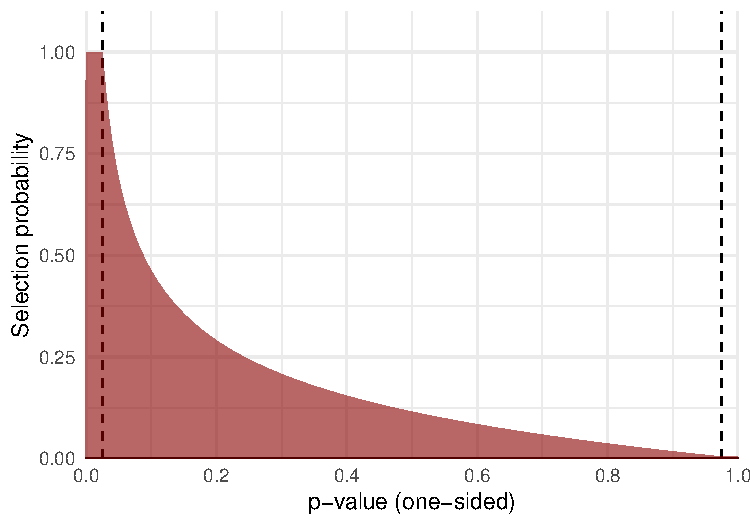
\includegraphics[width=0.49\linewidth]{beta-function-selection-models-with-dependent-effects_files/figure-latex/beta-functions-1} }\subfloat[Complex selection: $\lambda_1 = 0.5, \lambda_2 = 0.6$\label{fig:beta-functions-2}]{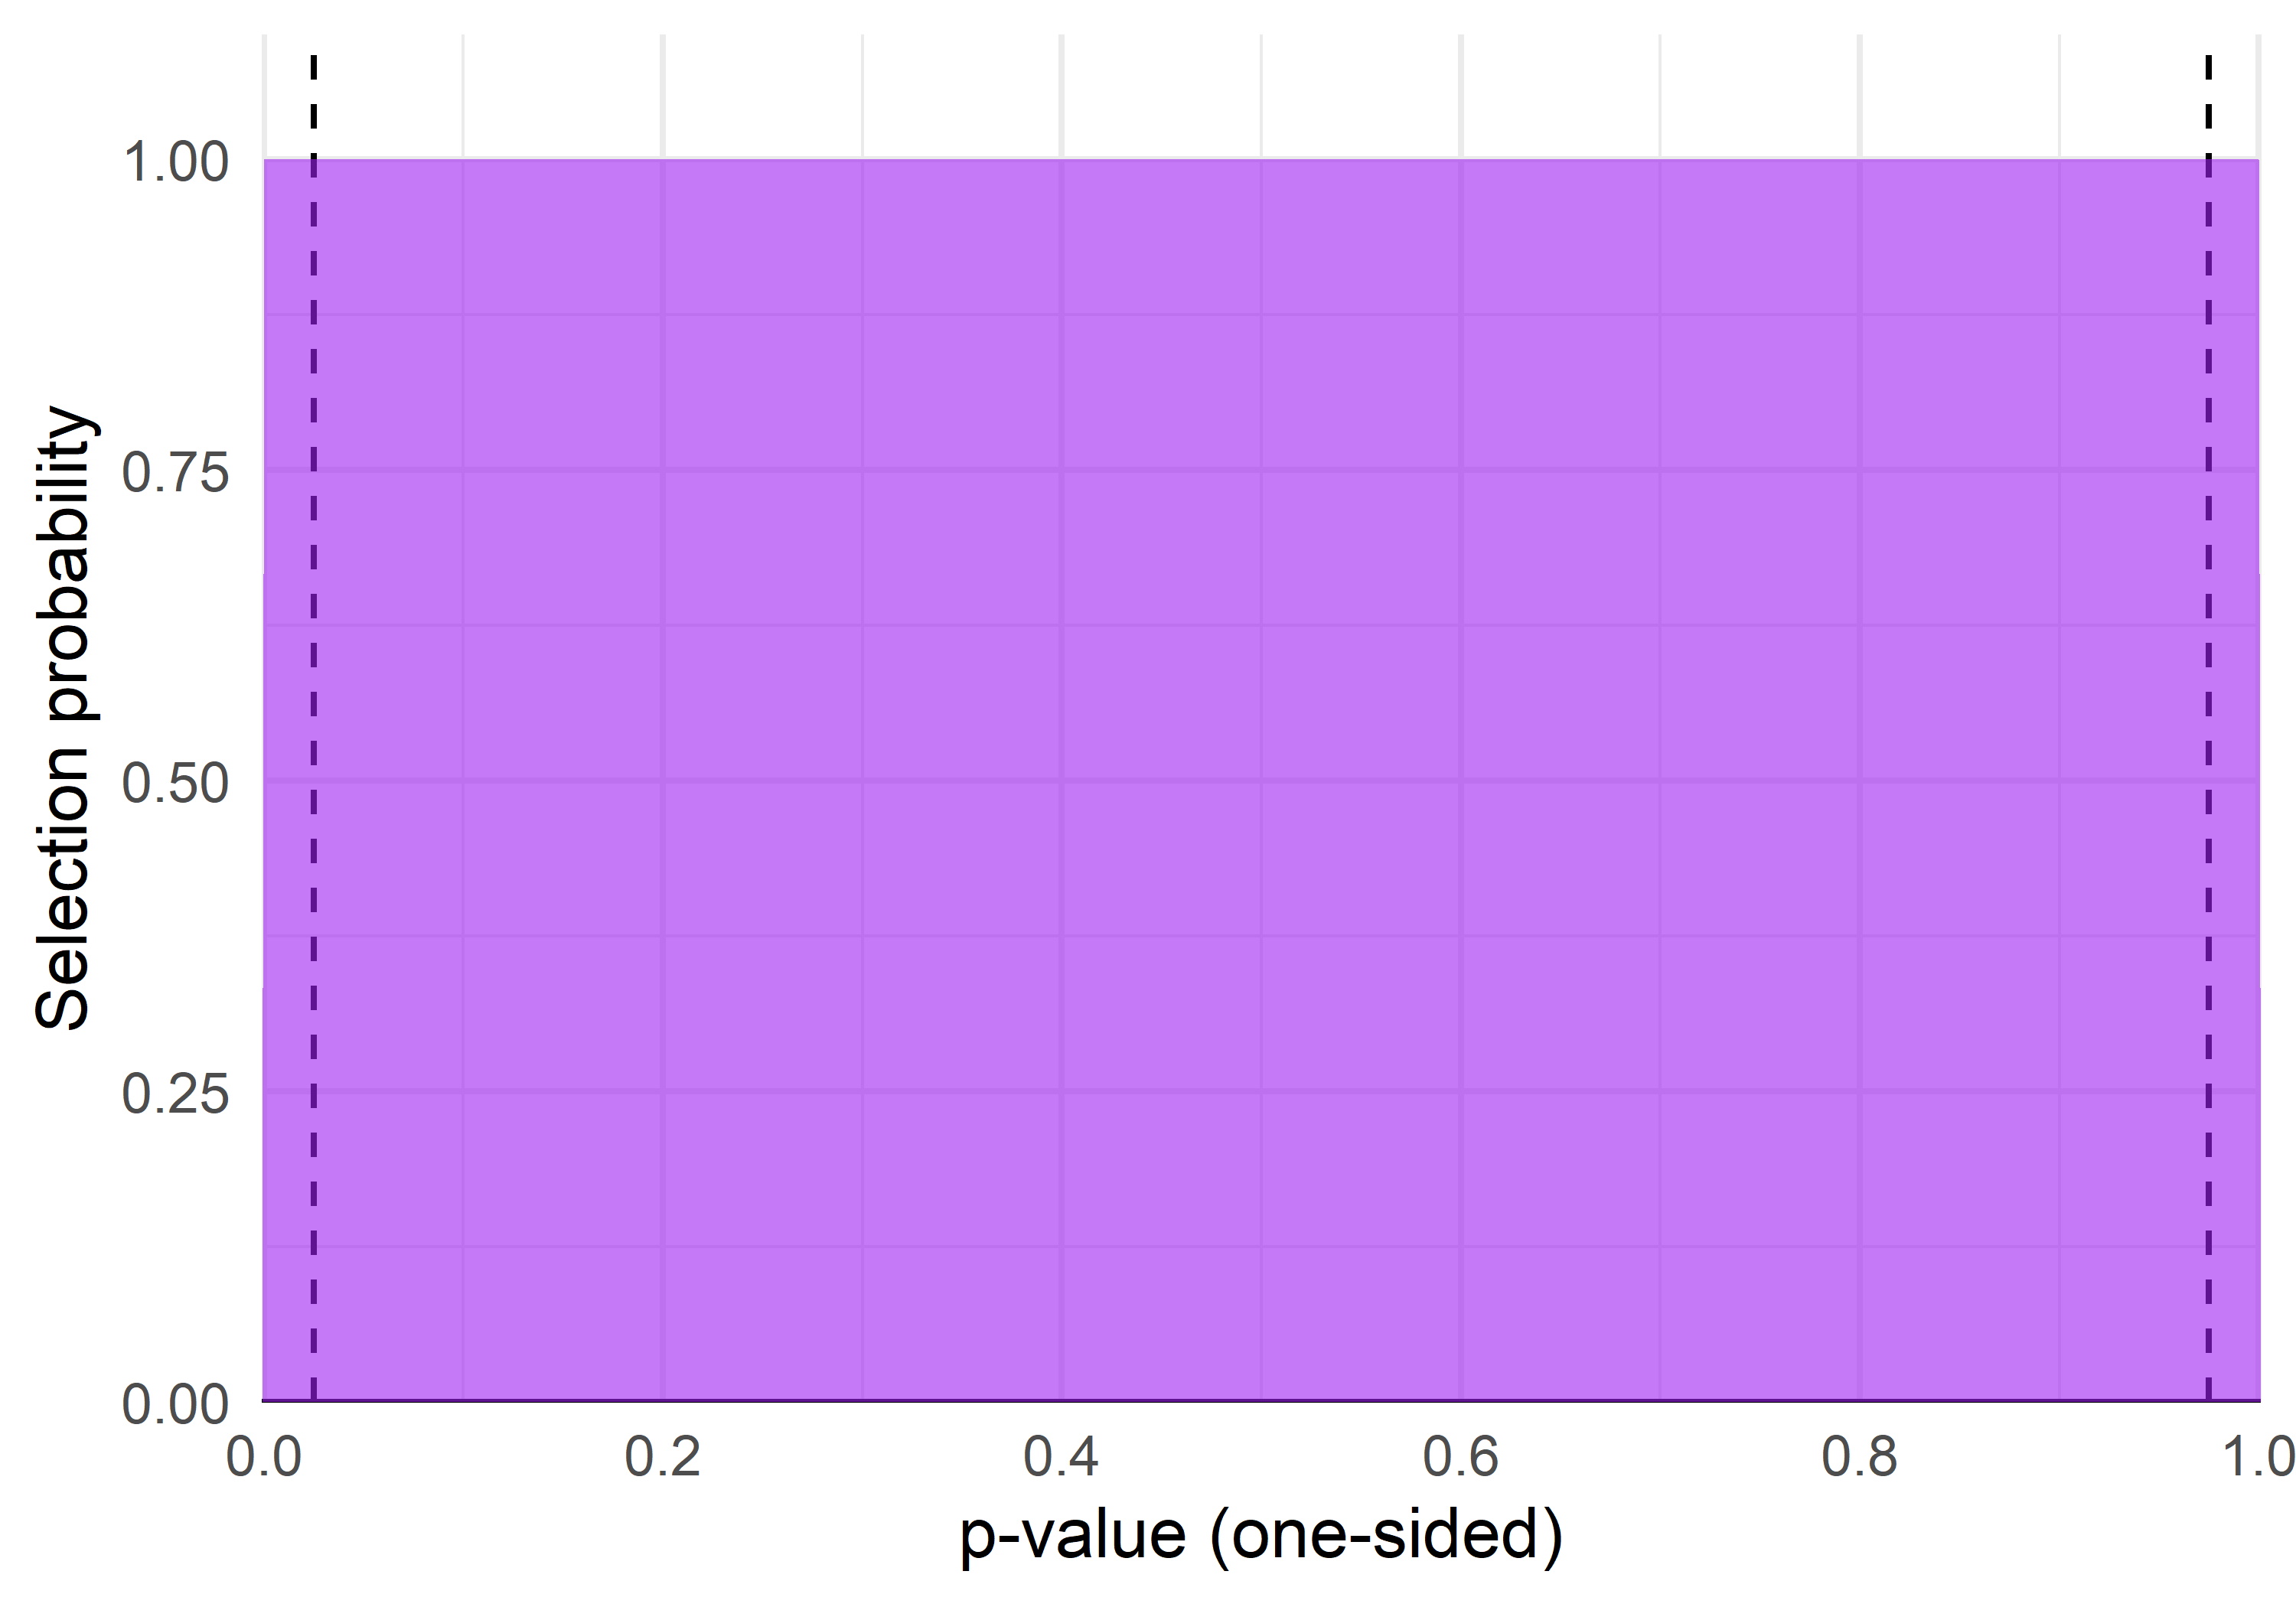
\includegraphics[width=0.49\linewidth]{beta-function-selection-models-with-dependent-effects_files/figure-latex/beta-functions-2} }\caption{Examples of beta density functions}\label{fig:beta-functions}
\end{figure}

\subsection{Distribution of observed effect size estimates}\label{distribution-of-observed-effect-size-estimates}

The combined model for the marginal density of an observed effect size estimate \(Y\) with standard error \(\sigma\) has the form
\begin{equation}
\label{eq:generic-selection}
f(Y = y | \sigma, \mathbf{x}) = \frac{1}{A(\mathbf{x}, \sigma; \boldsymbol\beta, \tau^2, \boldsymbol\lambda)} \times w\left(y, \sigma; \boldsymbol\lambda \right) \times \frac{1}{\sqrt{\tau^2 + \sigma^2}} \phi\left(\frac{y - \mathbf{x} \boldsymbol\beta}{\sqrt{\tau^2 + \sigma^2}}\right),
\end{equation}
where
\begin{equation}
\label{eq:generic-selection-A}
A(\mathbf{x}, \sigma; \boldsymbol\beta, \tau^2, \boldsymbol\lambda) =  \int_\mathbb{R} w\left(y, \sigma; \boldsymbol\lambda \right) \times  \frac{1}{\sqrt{\tau^2 + \sigma^2}}\phi\left(\frac{y - \mathbf{x}\boldsymbol\beta}{\sqrt{\tau^2 + \sigma^2}}\right) dy.
\end{equation}
For the beta-density selection process, the \(A(\mathbf{x}, \sigma; \boldsymbol\beta, \tau^2, \boldsymbol\lambda)\) term in the beta-density composite likelihood must be computed using numerical integration.
If \(w(y, \sigma; \boldsymbol\lambda) = 1\), then \(A(\mathbf{x}, \sigma; \boldsymbol\beta, \tau^2, \boldsymbol\lambda) = 1\) and there is no selective reporting. The density then reduces to the unweighted density of the evidence-generating process and the \(\boldsymbol\beta\) estimates from the adjusted beta function selection model will approximate those of the standard meta-analytic model.

\subsection{Estimation Method}\label{estimation-method}

We estimate model parameters using maximum composite marginal likelihood (CML), which treats each observed effect size estimate as if it were mutually independent, following established composite likelihood approaches (e.g., Cox \& Reid, 2004; Lindsay, 1988; Varin, 2008). Estimation proceeds by maximizing a weighted log-likelihood function defined over the marginal contributions of each observation, using reparameterizations of the variance and selection parameters. Confidence intervals are constructed using robust (sandwich-type) variance estimators based on study-level score contributions. A detailed explanation of CML methods is provided in our previous paper (Pustejovsky, Citkowicz, et al., 2025), and the exact expressions used for estimating the beta-density selection model are presented in APPENDIX.

\subsection{Bootstrap inference}\label{bootstrap-inference}

To improve inference accuracy with a limited number of studies, we also implement bootstrap procedures, which generate pseudo-samples through random resampling or reweighting of the original data. We considered several bootstrap methods designed to preserve the dependence structure across clusters, including the non-parametric clustered bootstrap, two-stage bootstrap (Field \& Welsh, 2007; Leeden, Meijer, \& Busing, 2008), and fractional random weight bootstrap (Rubin, 1981; Xu, Gotwalt, Hong, King, \& Meeker, 2020). Based on our prior work (Pustejovsky, Citkowicz, et al., 2025), which found that the two-stage bootstrap consistently outperformed the alternatives, we focus exclusively on this approach. Confidence intervals are then computed using standard bootstrap-based methods such as the percentile, basic, studentized, and bias-corrected-and-accelerated intervals (Davison \& Hinkley, 1997; Efron, 1987). These resampling-based procedures are particularly useful in small-sample contexts where sandwich estimators may perform poorly. APPENDIX provides further details about the bootstrap CI calculations.

\section{Empirical Example}\label{empirical-example}

To demonstrate the interpretation of the beta-density selection model in practice, we reanalyzed the data from a meta-analysis of the effects of science interventions on K--12 student science achievement, conducted by BSCS Science Learning (Taylor et al., 2018). The meta-analytic sample included findings from 96 studies with 292 effects. Approximately half of the studies contributed multiple effects per study, due to either multiple samples or multiple outcomes, leading to dependent effect sizes. Effect sizes were measured as standardized mean differences representing the effects of the interventions on student achievement outcomes, with positive effects corresponding to improvements in student achievement.

We conducted the analyses using R Version 4.4.3 (R Core Team, 2023).
We first used the \texttt{rma.uni()} function from the \texttt{metafor} package to fit a standard random-effects model based on an independent effects working model with random effects for each study (Viechtbauer, 2010), with standard errors clustered by study.
The overall estimate of the average effect using the unadjusted model is 0.44, cluster-robust 95\% CI {[}0.34, 0.54{]}, which is significantly different from zero \((p <0.001)\).
The unadjusted estimate of heterogeneity is \(\tau = 0.38\).

To adjust for selective reporting, we used the \texttt{selection\_model()} function from the \texttt{metaselection} package to fit the beta-density selection model (with default truncation thresholds of \(\alpha_1 = .025, \alpha_2 = .975\)) along with two step-function selection models (Pustejovsky, Joshi, \& Citkowicz, 2025). Both selection models are based on an independent effects working model with random effects for each study and account for dependent effects using robust variance estimation, clustering by study. For the step-function models, we estimated both a single-step model with a threshold at \(\alpha_1 = 0.025\) and a two-step model with thresholds at \(\alpha_1 = .025\) and \(\alpha_2 = .5\).

\begin{table}
\centering
\caption{\label{tab:science-learning-res}Selection model parameter estimates fit to science intervention effects from Taylor et al. (2018)}
\centering
\begin{tabular}[t]{lllllll}
\toprule
\multicolumn{1}{c}{ } & \multicolumn{2}{c}{Beta density} & \multicolumn{2}{c}{One-step} & \multicolumn{2}{c}{Two-step} \\
\cmidrule(l{3pt}r{3pt}){2-3} \cmidrule(l{3pt}r{3pt}){4-5} \cmidrule(l{3pt}r{3pt}){6-7}
Parameter & Est. (SE) & 95\% CI & Est. (SE) & 95\% CI & Est. (SE) & 95\% CI\\
\midrule
\addlinespace[0.3em]
\multicolumn{7}{l}{\textbf{Summary meta-analysis}}\\
\hspace{1em}$\beta_0$ & 0.33 (0.12) & {}[0.10, 0.56] & 0.58 (0.06) & {}[0.46, 0.71] & 0.49 (0.07) & {}[0.35, 0.64]\\
\hspace{1em}$\tau$ & 0.46 (0.17) & {}[0.39, 0.54] & 0.40 (0.21) & {}[0.32, 0.49] & 0.43 (0.19) & {}[0.36, 0.52]\\
\hspace{1em}$\lambda_1$ & 1.10 (0.14) & {}[0.83, 1.46] & 2.21 (0.26) & {}[1.34, 3.65] & 1.93 (0.26) & {}[1.16, 3.22]\\
\hspace{1em}$\lambda_2$ & 1.55 (0.17) & {}[1.11, 2.17] &  &  & 1.08 (0.43) & {}[0.47, 2.49]\\
\addlinespace[0.3em]
\multicolumn{7}{l}{\textbf{Moderator analysis}}\\
\hspace{1em}$\beta_0$ & 0.21 (0.24) & {}[-0.27, 0.69] & 0.51 (0.11) & {}[0.29, 0.74] & 0.40 (0.15) & {}[0.10, 0.70]\\
\hspace{1em}$\beta_1$ & 0.14 (0.18) & {}[-0.22, 0.50] & 0.10 (0.13) & {}[-0.16, 0.35] & 0.12 (0.15) & {}[-0.18, 0.42]\\
\hspace{1em}$\tau$ & 0.46 (0.17) & {}[0.40, 0.55] & 0.40 (0.21) & {}[0.32, 0.49] & 0.43 (0.18) & {}[0.36, 0.52]\\
\hspace{1em}$\lambda_1$ & 1.09 (0.15) & {}[0.82, 1.46] & 2.22 (0.26) & {}[1.34, 3.67] & 1.93 (0.26) & {}[1.16, 3.22]\\
\hspace{1em}$\lambda_2$ & 1.58 (0.18) & {}[1.11, 2.24] &  &  & 1.05 (0.43) & {}[0.45, 2.47]\\
\bottomrule
\multicolumn{7}{l}{\rule{0pt}{1em}\textit{Note: }}\\
\multicolumn{7}{l}{\rule{0pt}{1em}Est. = estimate; SE = cluster-robust standard error; CI = cluster-robust confidence interval.}\\
\end{tabular}
\end{table}

The upper panel of Table \ref{tab:science-learning-res} reports parameter estimates from all three models, along with cluster-robust standard errors and 95\% confidence intervals.
Across the three selection models, the estimated average effect sizes are all positive and significant, but they vary in magnitude and interpretation. Compared to the unadjusted model, the average adjusted effect is 25\% smaller when using the beta-density selection model (\(ES\) = 0.33), versus 32\% larger when using the single-step model (\(ES\) = 0.58) and 12\% larger when using the two-step selection model (\(ES\) = 0.49).
These differences are due to differences in the form of the selection curve estimated from each model specification, as depicted in figure \ref{fig:science-selection-curves}.
The beta-density model estimates of \(\lambda_1\) and \(\lambda_2\) imply that positive but non-significant results are slightly more likely to be reported compared to affirmative results, but that negative effects are increasingly less likely to be be reported.
On balance, this leads to an adjusted average effect size estimate that is smaller than under the unadjusted random effects model.
In contrast, the step-function models both estimate that non-significant results are more likely to be reported compared to affirmative results, leading to upward adjustment in the average effect size.

\begin{figure}[tb]
\includegraphics[width=0.75\linewidth]{beta-function-selection-models-with-dependent-effects_files/figure-latex/science-selection-curves-1} \caption{Estimated selection functions based on beta density, one-step, and two-step selection models}\label{fig:science-selection-curves}
\end{figure}

A key advantage of selection models over other methods for diagnosing and adjusting for selective reporting bias is that they allow for inclusion of potential moderator variables as predictors of average effect size. This feature allows meta-analysts to distinguish selective reporting bias from systematic variation in effect sizes that could be explained by primary study characteristics.
Past work has demonstrated that evaluations of educational interventions tend to produce larger effects on assessments developed by study authors or developers of the intervention (i.e., non-independent groups) than on assessments developed by groups independent of the evaluation (Wolf \& Harbatkin, 2023).
We investigated whether this pattern holds in the BSCS Science Learning meta-analysis data, which includes an indicator for assessment type, equal to one for assessments developed by non-independent groups and equal to zero otherwise.

We reran all four models using assessment type as a moderator (Taylor et al., 2018), with assessments developed by independent groups as the reference category.
Based on a random effects meta-regression without adjustment for selective reporting, assessments developed by independent groups produced an average effect size of 0.38, 95\% CI {[}0.14, 0.62{]}.
The average effect on assessments developed by non-independent groups was larger by 0.09 SD, 95\% CI {[}-0.17, 0.35{]}, which was not statistically distinct from zero \((p = 0.495)\).
The unadjusted estimate of heterogeneity is \(\tau = 0.38\), just as in the summary meta-analysis.

The lower panel of Table \ref{tab:science-learning-res} reports parameter estimates from the corresponding selection models that include assessment type as a predictor.
The \(\beta_1\) coefficient estimates represent differences in average effects between non-independent and independent assessment developers, which were all non-significant and similar in magnitude to the difference based on the unadjusted model.
However, the selection models lead to different about the average effects on independently developed assessments.
The estimate from the beta-density model is not statistically distinct from zero and is smaller than the estimate from the unadjusted random effects meta-regression.
In contrast, the estimated average effects from the step-function selection models are both statistically significant and larger than the estimate from the unadjusted model.
Selection parameter estimates are very similar to the estimates from the corresponding summary meta-analysis models.

The model estimates reveal some key differences between the selection models. In this dataset, the beta-density selection model adjusts the estimates downward---so much so in the moderator analysis that neither estimate remains statistically significant. The step-function selection model, on the other hand, adjusts the estimates upward, though the adjustment is minimal when using the two-step model.
These differences suggest that the models' distinct assumptions about the shape of the selection function may lead to varying results. Specifically, the beta-density selection model, which allows for a smooth, continuous function, appears to be capturing a pattern of selection that differs from the discrete thresholds assumed by the step-function selection model.
To investigate this, we conducted simulations across a wide range of conditions. The simulations will allow us to draw firmer conclusions about the comparative performance of these methods, including their robustness to misspecification of the selection function.

\section{Simulation Methods}\label{simulation-methods}

We conducted Monte Carlo simulation studies to assess the performance of the marginal beta-density selection model and to investigate whether the form of the selection mechanism matters.
The simulations covered a wide range of conditions in which primary studies contributed multiple, statistically dependent effect size estimates.
We compared the new model to three exiting methods: (1) a new version of the correlated hierarchical effects model with inverse sampling-covariance weights (CHE-ISCW), which accounts for dependency but not selective reporting (Chen \& Pustejovsky, 2024); (2) the PET-PEESE method, which addresses selective reporting and has been adapted to handle dependent data structures (Stanley \& Doucouliagos, 2014); and (3) our recently developed step-function selection model that accounts for both selective reporting and dependent effects (Pustejovsky, Citkowicz, et al., 2025).
We evaluated the model estimates based on convergence rates, bias, accuracy, and confidence interval coverage for estimating the average effect size from the unselected distribution. Bootstrap confidence intervals were assessed under a narrower set of conditions to limit computational burden.
Simulations were conducted in R Version 4.4.0 (R Core Team, 2023) using the high-throughput computing cluster at the University of Wisconsin--Madison (Center for High Throughput Computing, 2006).
The code relied on several R packages, including metafor (Viechtbauer, 2010), clubSandwich (Pustejovsky, 2024), simhelpers (Joshi \& Pustejovsky, 2024), optimx (Nash \& Varadhan, 2011), and tidyverse (Wickham et al., 2019).

\subsection{Data generation}\label{data-generation}

We generated simulated data using an approach similar to Pustejovsky, Citkowicz, et al. (2025), with the key difference that effect size estimates were selected for inclusion based on the beta-density selection model. For each simulated meta-analysis, we generated a pool of primary studies using a CHE model, with effect size estimates selected for inclusion according to probabilities defined by the beta-density selection model. Each study followed a two-group design, with sample sizes and numbers of effect sizes per study drawn from an empirical distribution based on the What Works Clearinghouse database. We generated outcome correlations across studies by sampling from a beta distribution with mean \(\rho\) and standard deviation 0.05, then assumed a constant correlation between pairs of outcomes within a study.

Within each study, we simulated a study-level average effect size \(\delta_j\) from a normal distribution with mean \(\mu\) and variance \(\tau^2_B\), then generated individual effect size parameters from a normal distribution centered at \(\delta_j\) with variance \(\omega^2\). Using these parameters, we drew multivariate normal outcomes for participants equally divided into treatment and control groups and computed standardized mean differences with Hedges's \(g\) small sample bias correction. One-sided \(p\)-values were computed for each effect size, and individual effect sizes were then selected for inclusion in the dataset, with selection probabilities determined by the beta-density selection model with parameters \(\lambda_1,\lambda_2\).
We repeated this process until the simulated meta-analytic dataset included at total of \(J\) studies with at least one observed result.

\subsection{Estimation methods}\label{estimation-methods}

We estimated the beta-density selection model using the CML approach described in Section \ref{estimation-methods}. We calculated cluster-robust standard errors using large-sample sandwich formulas. For a subset of simulation conditions, we also examined percentile, basic, studentized, and bias-corrected-and-accelerated confidence intervals based on the two-stage bootstrap. To maintain computational feasibility, we used \(B = 399\) bootstrap replications of each estimator.

We compared the performance of the beta-density selection model to three other methods. First, we estimated a summary meta-analysis model using the CHE-ISCW approach proposed by Chen and Pustejovsky (2024), which accounts for effect size dependence but does not adjust for selective reporting. This method fits a CHE working model, but it allocates more weight to studies with smaller sampling variances by using generalized least squares with weighting matrices that are the inverse of the variance-covariance matrix of the sampling errors only. We assumed a correlation of 0.80, which leads to a degree of misspecification when the average correlation used in the data-generating process differs from 0.80. We computed confidence intervals for the average effect size using cluster-robust variance estimation with the CR2 small-sample correction and Satterthwaite degrees of freedom.

Second, we estimated a variation of the PET/PEESE model originally proposed by Stanley and Doucouliagos (2014), adapted to handle dependent effect sizes. The PET model regresses effect size estimates on their standard errors, while the PEESE model uses sampling variances instead. Both models assume normally distributed errors with a correlation of 0.80 and were estimated using the same procedure as the CHE-ISCW model, including using CR2 cluster-robust standard errors. Following Stanley and Doucouliagos (2014), we used the PET estimate if it was not statistically distinguishable from zero at an \(\alpha\)-level of 0.10; otherwise, we used the PEESE estimate.

Third, we estimated the step-function selection model using the CML approach described in Pustejovsky, Citkowicz, et al. (2025).
We estimated two step-function selection models: (1) a one-step selection model with a single step at \(\alpha_1 = 0.025\), and (2) a two-step selection model with steps at \(\alpha_1 = 0.025\) and \(\alpha_2 = 0.500\).
Like the beta-density selection model, the one-step and two-step models are \(p\)-value selection models designed to address selective reporting, they are models for the marginal rather than joint distribution of estimates within studies, and they use cluster-robust variance estimation or bootstrapping to account for dependency.
The main distinction between the step-function and beta-density selection models lies in the form of the selection mechanism. By fitting the one-step and two-step selection models to data simulated under a beta-density selection process, we can assess how robust these models are to misspecification of the selection function and whether the form of selection affects their performance.

\subsection{Experimental design}\label{experimental-design}

We examined performance across a range of simulation conditions, summarized in Table \ref{tab:sim-design}. Manipulated parameters included overall average standardized mean difference (\(\mu\)), between-study heterogeneity (\(\tau_B\)), ratio of within- to between-study heterogeneity (\(\omega^2 / \tau^2\)), average correlation between outcomes (\(\rho\)), probability of selection for non-affirmative results (\(\lambda_1, \lambda_2\)), and number of observed studies (\(J\)). The full simulation crossed all parameter values for a total of \(4 \times 4 \times 2 \times 2 \times 5 \times 4 = 1,280\) conditions. For the more computationally intensive bootstrap simulations, we limited the design to a smaller subset of \(4 \times 3 \times 2 \times 1 \times 3 \times 3 = 216\) conditions, focusing on smaller meta-analyses and reducing values for factors where results were stable (e.g., \(\tau = 0.30\)). For each condition, we generated 2,000 replications.

\begin{table}
\centering
\caption{\label{tab:sim-design}Parameter values examined in the simulation study}
\centering
\begin{tabular}[t]{>{\raggedright\arraybackslash}p{2.5in}>{\raggedright\arraybackslash}p{1.75in}>{\raggedright\arraybackslash}p{1.75in}}
\toprule
Parameter & Full Simulation & Bootstrap Simulation\\
\midrule
Overall average SMD ($\mu$) & 0.0, 0.2, 0.4, 0.8 & 0.0, 0.2, 0.4, 0.8\\
Between-study heterogeneity ($\tau$) & 0.05, 0.15, 0.30, 0.45 & 0.05, 0.15, 0.45\\
Heterogeneity ratio ($\omega^2 / \tau^2$) & 0.0, 0.5 & 0.0, 0.5\\
Average correlation between outcomes ($\rho$) & 0.40, 0.80 & 0.80\\
Probability of selection for non-affirmative effects ($\lambda_1, \lambda_2$) & (0.01, 0.90), (0.20, 0.90), (0.50, 0.90), (0.80, 0.90), (1.00, 1.00) & (0.20, 0.90), (0.50, 0.90), (1.00, 1.00)\\
\addlinespace
Number of observed studies ($J$) & 15, 30, 60, 90 & 15, 30, 60\\
\bottomrule
\end{tabular}
\end{table}

In the full simulation, we varied \(\mu\) from 0.0 to 0.80, reflecting the range of effects observed in a large-scale review of education randomized controlled trials (Kraft, 2020), and \(\tau\) from 0.05 (minimal heterogeneity) to 0.45 (substantial heterogeneity). Within-study heterogeneity was specified relative to between-study heterogeneity using a ratio of \(\omega^2 / \tau^2\) equal to 0 (no within-study heterogeneity) or 0.5.

To assess the impact of working model misspecification, we manipulated the average within-study correlation \(\rho\) across two levels: 0.80 (the default used in RVE software and correctly specified when \(\rho = 0.80\)) and 0.40 (inducing misspecification in the CHE-ISCW and PET-PEESE working models).

Selective reporting was modeled as the probability of selecting non-affirmative results based on the parameters of the beta-density. We considered five levels of selective reporting, including no selection (\(\lambda_1 = 1.00, \lambda_2 = 1.00\)), weak selection (\(\lambda_1 = 0.80, \lambda_2 = 0.90\)), moderate selection (\(\lambda_1 = 0.50, \lambda_2 = 0.90\)), strong selection (\(\lambda_1 = 0.20, \lambda_2 = 0.90\)), and very strong selection (\(\lambda_1 = 0.01, \lambda_2 = 0.90\)).

We varied the number of observed studies (\(J\)) from 15 to 90, covering the typical size of meta-analyses in education and psychology (Tipton, Pustejovsky, \& Ahmadi, 2019).
We simulated primary study sample sizes based on the empirical distribution in the What Works Clearinghouse database. The sample sizes in the database ranged from 37 to 2,295 with a median of 211, and the number of effect sizes ranged from 1 to 48 with a median of 3.\footnote{
  Pustejovsky, Citkowicz, et al. (2025) included a condition in which the primary study sample sizes were divided by three to represent smaller studies, such as those in psychology lab settings. However, the simulation results for this condition were similar to those from the empirical distribution condition, so we have omitted it from the current simulations.}

\subsection{Performance criteria}\label{performance-criteria}

We evaluated each method's performance in terms of convergence rates, bias, scaled root mean-squared error (RMSE), and 95\% confidence interval coverage for the overall effect size \(\mu\).
Bias reflects systematic deviation from the true parameter value, while RMSE captures both bias and sampling variability.
To account for expected reductions in RMSE with more studies, we scaled RMSE by \(\sqrt{J}\).
Bias and scaled RMSE were calculated after winsorizing to limit the influence of extreme outliers, using fences set at 2.5 times the interquartile range beyond the 25th and 75th percentiles.

For confidence intervals based on cluster-robust variance estimation, we defined coverage as the proportion of intervals that contained the true parameter value. For bootstrap intervals, we used \(B = 399\) replicates per simulation due to computational limits---fewer than ideal for applied use. To estimate practical coverage rates, we followed an approach similar to Boos and Zhang (2000): we calculated coverage for smaller subsamples (\(B = 49, 99, 199, 299\)) randomly selected without replacement from the full set of \(B = 399\) bootstraps, fit a regression of coverage on \(1/B\), and used the intercept to extrapolate expected coverage for \(B = 1999\).

\section{Simulation Results}\label{simulation-results}

\begin{verbatim}
## # A tibble: 3,840 x 39
##    mean_smd   tau cor_mu delta_1     m omega delta_2 bootstrap_condition
##       <dbl> <dbl>  <dbl>   <dbl> <dbl> <dbl>   <dbl> <chr>              
##  1      0    0.05    0.4    0.01    90 0         0.9 none               
##  2      0    0.05    0.4    0.01    90 0         0.9 none               
##  3      0    0.05    0.4    0.01    90 0         0.9 none               
##  4      0.8  0.45    0.4    0.5     30 0.318     0.9 none               
##  5      0.8  0.45    0.4    0.5     30 0.318     0.9 none               
##  6      0.8  0.45    0.4    0.5     30 0.318     0.9 none               
##  7      0    0.15    0.4    0.2     60 0.106     0.9 none               
##  8      0    0.15    0.4    0.2     60 0.106     0.9 none               
##  9      0    0.15    0.4    0.2     60 0.106     0.9 none               
## 10      0.8  0.45    0.4    0.5     15 0.318     0.9 none               
## # i 3,830 more rows
## # i 31 more variables: model_estimator <chr>, model <chr>, estimator <fct>,
## #   param <chr>, K_coverage <int>, width_winsor_pct <dbl>,
## #   width_winsor_pct_mcse <dbl>, coverage <dbl>, coverage_mcse <dbl>,
## #   width <dbl>, width_mcse <dbl>, K_relvar <int>, est_winsor_pct <dbl>,
## #   est_winsor_pct_mcse <dbl>, var_winsor_pct <dbl>, var_winsor_pct_mcse <dbl>,
## #   rel_bias_var <dbl>, rel_bias_var_mcse <dbl>, rel_rmse_var <dbl>, ...
\end{verbatim}

We organize our simulation results into two parts. First, we compare the performance of the beta-density selection model to the CHE-ISCW and PET/PEESE approaches. Specifically, we compare the bias and accuracy of the average effect size, the coverage rates of 95\% confidence intervals of the average effect size, and the estimation of the marginal variance of the effect size distribution. Second, we compare the performance of the beta-density selection model to the one-step and two-step selection models to assess the robustness of these models to misspecification of the selection function.

\subsection{Beta-Density Selection Model Compared to CHE-ISCW and PET/PEESE}\label{beta-density-selection-model-compared-to-che-iscw-and-petpeese}

The CHE-ISCW and PET/PEESE approaches had perfect convergence rates, producing results for every replication in every condition. The beta-density selection model exhibited very high convergence rates, with an average rate of 99.60\%; the lowest convergence rates occurred under conditions with the lowest degree of heterogeneity \(\tau = 0.05\). Supplementary Figure \ref{fig:convergence-rates-main} depicts the range of convergence rates of the beta-density selection model.

\subsubsection{Bias}\label{bias}

\begin{sidewaysfigure}
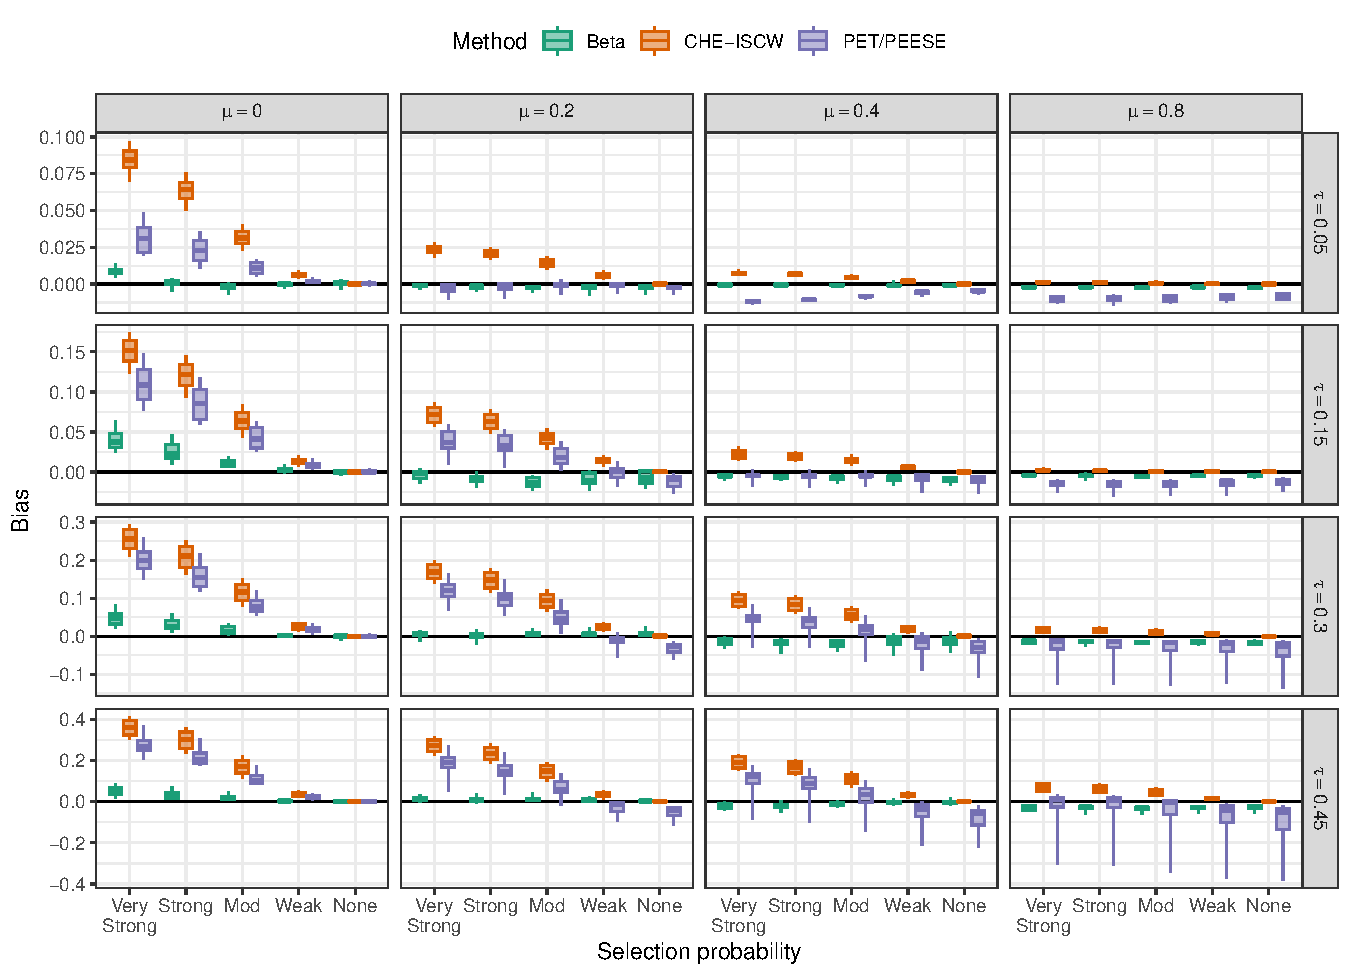
\includegraphics{beta-function-selection-models-with-dependent-effects_files/figure-latex/mu-bias-main-1} \caption{Bias of the average effect size by method, selection probability, average SMD, and between-study heterogeneity}\label{fig:mu-bias-main}
\end{sidewaysfigure}

Figure \ref{fig:mu-bias-main} shows the bias for each method of estimating the average effect size (vertical axis) as a function of selective reporting strength (horizontal axis), average effect size (grid column), and between-study heterogeneity (\(\tau\), grid row). Each box plot summarizes variation in bias across the remaining simulation factors: the heterogeneity ratio, the correlation between effect size estimates, and the number of observed studies. Note that the vertical axis scale differs by grid row, reflecting how some methods' bias is more sensitive to the level of heterogeneity.

The beta-density selection model has negligible to small bias across all conditions, ranging from -0.06 to 0.09. Its bias was essentially zero for all conditions when the average effect size is non-zero or when selective reporting is weak or absent. Bias was largest when selective reporting is very strong, average effect size is zero, and heterogeneity is large.

In contrast, bias for the comparison methods ranged from 0 to 0.41 for CHE-ISCW and -0.38 to 0.37 for PET/PEESE. Both methods are generally biased when selective reporting is present.
For CHE-ISCW, which does not directly adjust for selective reporting, bias was closest to zero when average effect size is large \((\mu = 0.8)\) and heterogeneity is low \((\tau \leq 0.15)\).
This result is not surprising because the large average effect size and low heterogeneity mean that the vast majority of simulated results are statistically significant, leaving little opportunity for the selection mechanism to operate.
For PET/PEESE, which uses a regression adjustment to account for possible selective reporting, bias was closest to zero when average effect size is moderate \((\mu = 0.4)\) and heterogeneity is low \((\tau = 0.15)\).
For both comparison methods, bias grows stronger when selection is stronger, when average effect size is smaller, and when heterogeneity is larger.
Bias is generally less pronounced for PET/PEESE than for CHE-ISCW.

\subsubsection{Scaled RMSE}\label{scaled-rmse}

\begin{sidewaysfigure}
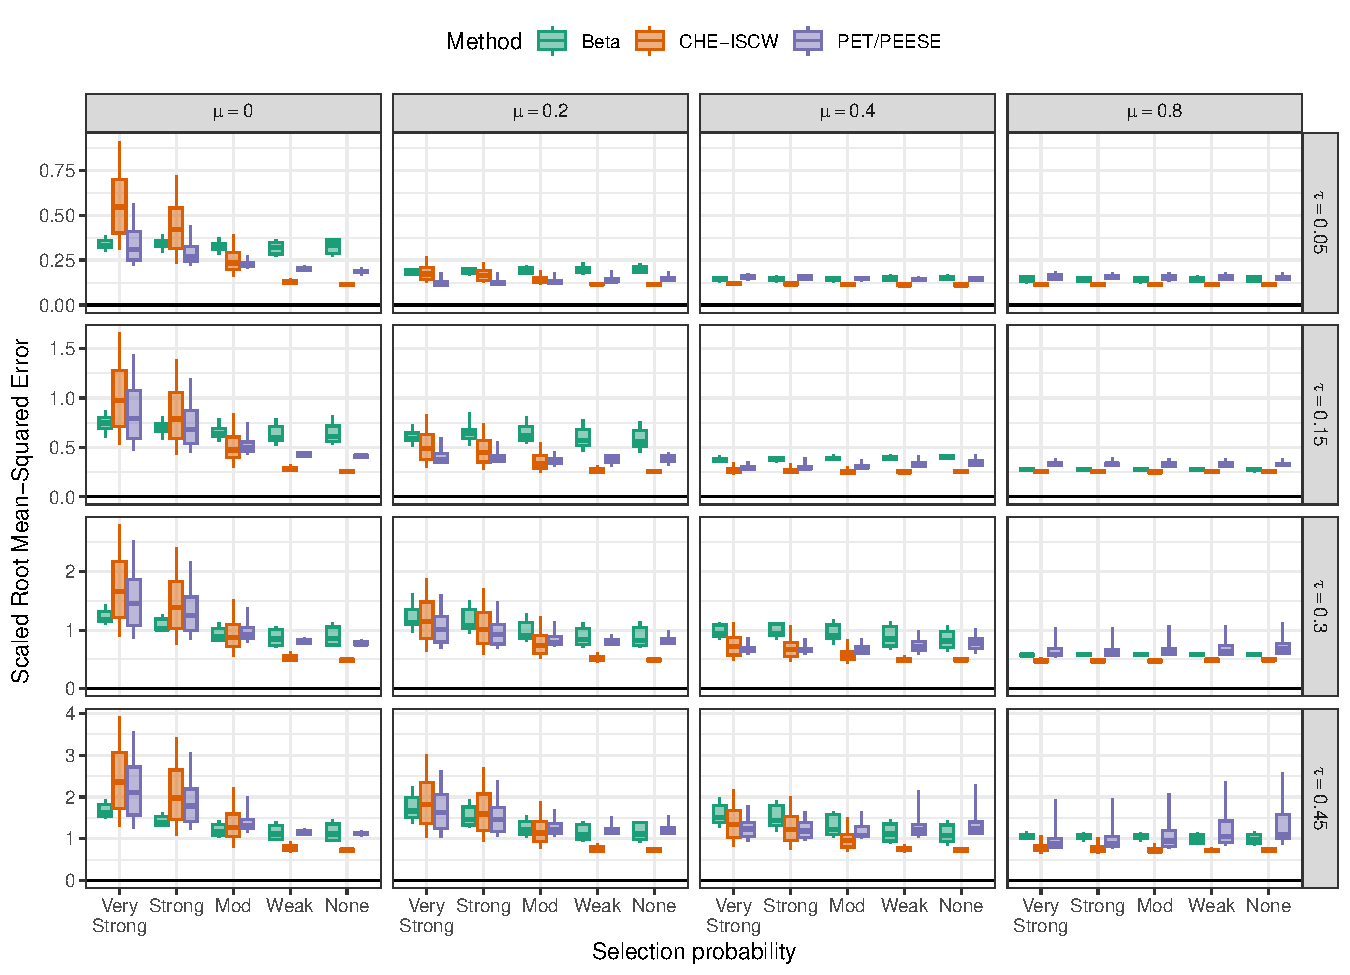
\includegraphics{beta-function-selection-models-with-dependent-effects_files/figure-latex/mu-rmse-main-1} \caption{Scaled root mean-squared error of the average effect size by method, selection probability, average SMD, and between-study heterogeneity}\label{fig:mu-rmse-main}
\end{sidewaysfigure}

Scaled RMSE captures both bias and variability, providing an overall measure of inaccuracy. Figure \ref{fig:mu-rmse-main}, constructed in the same format as Figure \ref{fig:mu-bias-main}, shows the scaled RMSE for each method of estimating the average effect size. Additional detail is provided in Figures \ref{fig:rmse-CHE-Beta-main} and \ref{fig:rmse-PET-Beta-main} in Appendix \ref{mu-simulation-results-main}, which plot the ratio of RMSEs for each pair of methods to compare their relative accuracy.

Taken together, the figures indicate that no single method achieves the lowest RMSE across all conditions. Instead, each method reflects different bias--variance trade-offs.
The beta-density selection model generally outperforms the others---achieving lower RMSE---when selective reporting is strong or very strong, average effect size is small \((\mu \leq 0.2)\), and heterogeneity is moderate to large \((\tau \geq 0.3)\).
CHE-ISCW consistently has the lowest RMSE when selective reporting is weak or absent.
PET/PEESE performs best when selective reporting is strong to very strong, average effect is small \((\mu \leq 0.2)\), and heterogeneity is low \((\tau \leq 0.15)\).

These bias--variance trade-offs stem from the fact that CHE-ISCW, which does not explicitly adjust for selective reporting, is more prone to bias when selection is present. In contrast, the beta-density selection model tends to produce smaller biases under such conditions. However, when selective reporting is weak or absent, CHE-ISCW is more precise than the methods that adjust for selective reporting (i.e., the beta-density selection model and PET/PEESE). Under those conditions, the added variability introduced by estimating a selection model or PET/PEESE adjustment outweighs the minimal reduction in bias they provide.

\subsubsection{Confidence Interval Coverage}\label{confidence-interval-coverage}

\begin{sidewaysfigure}
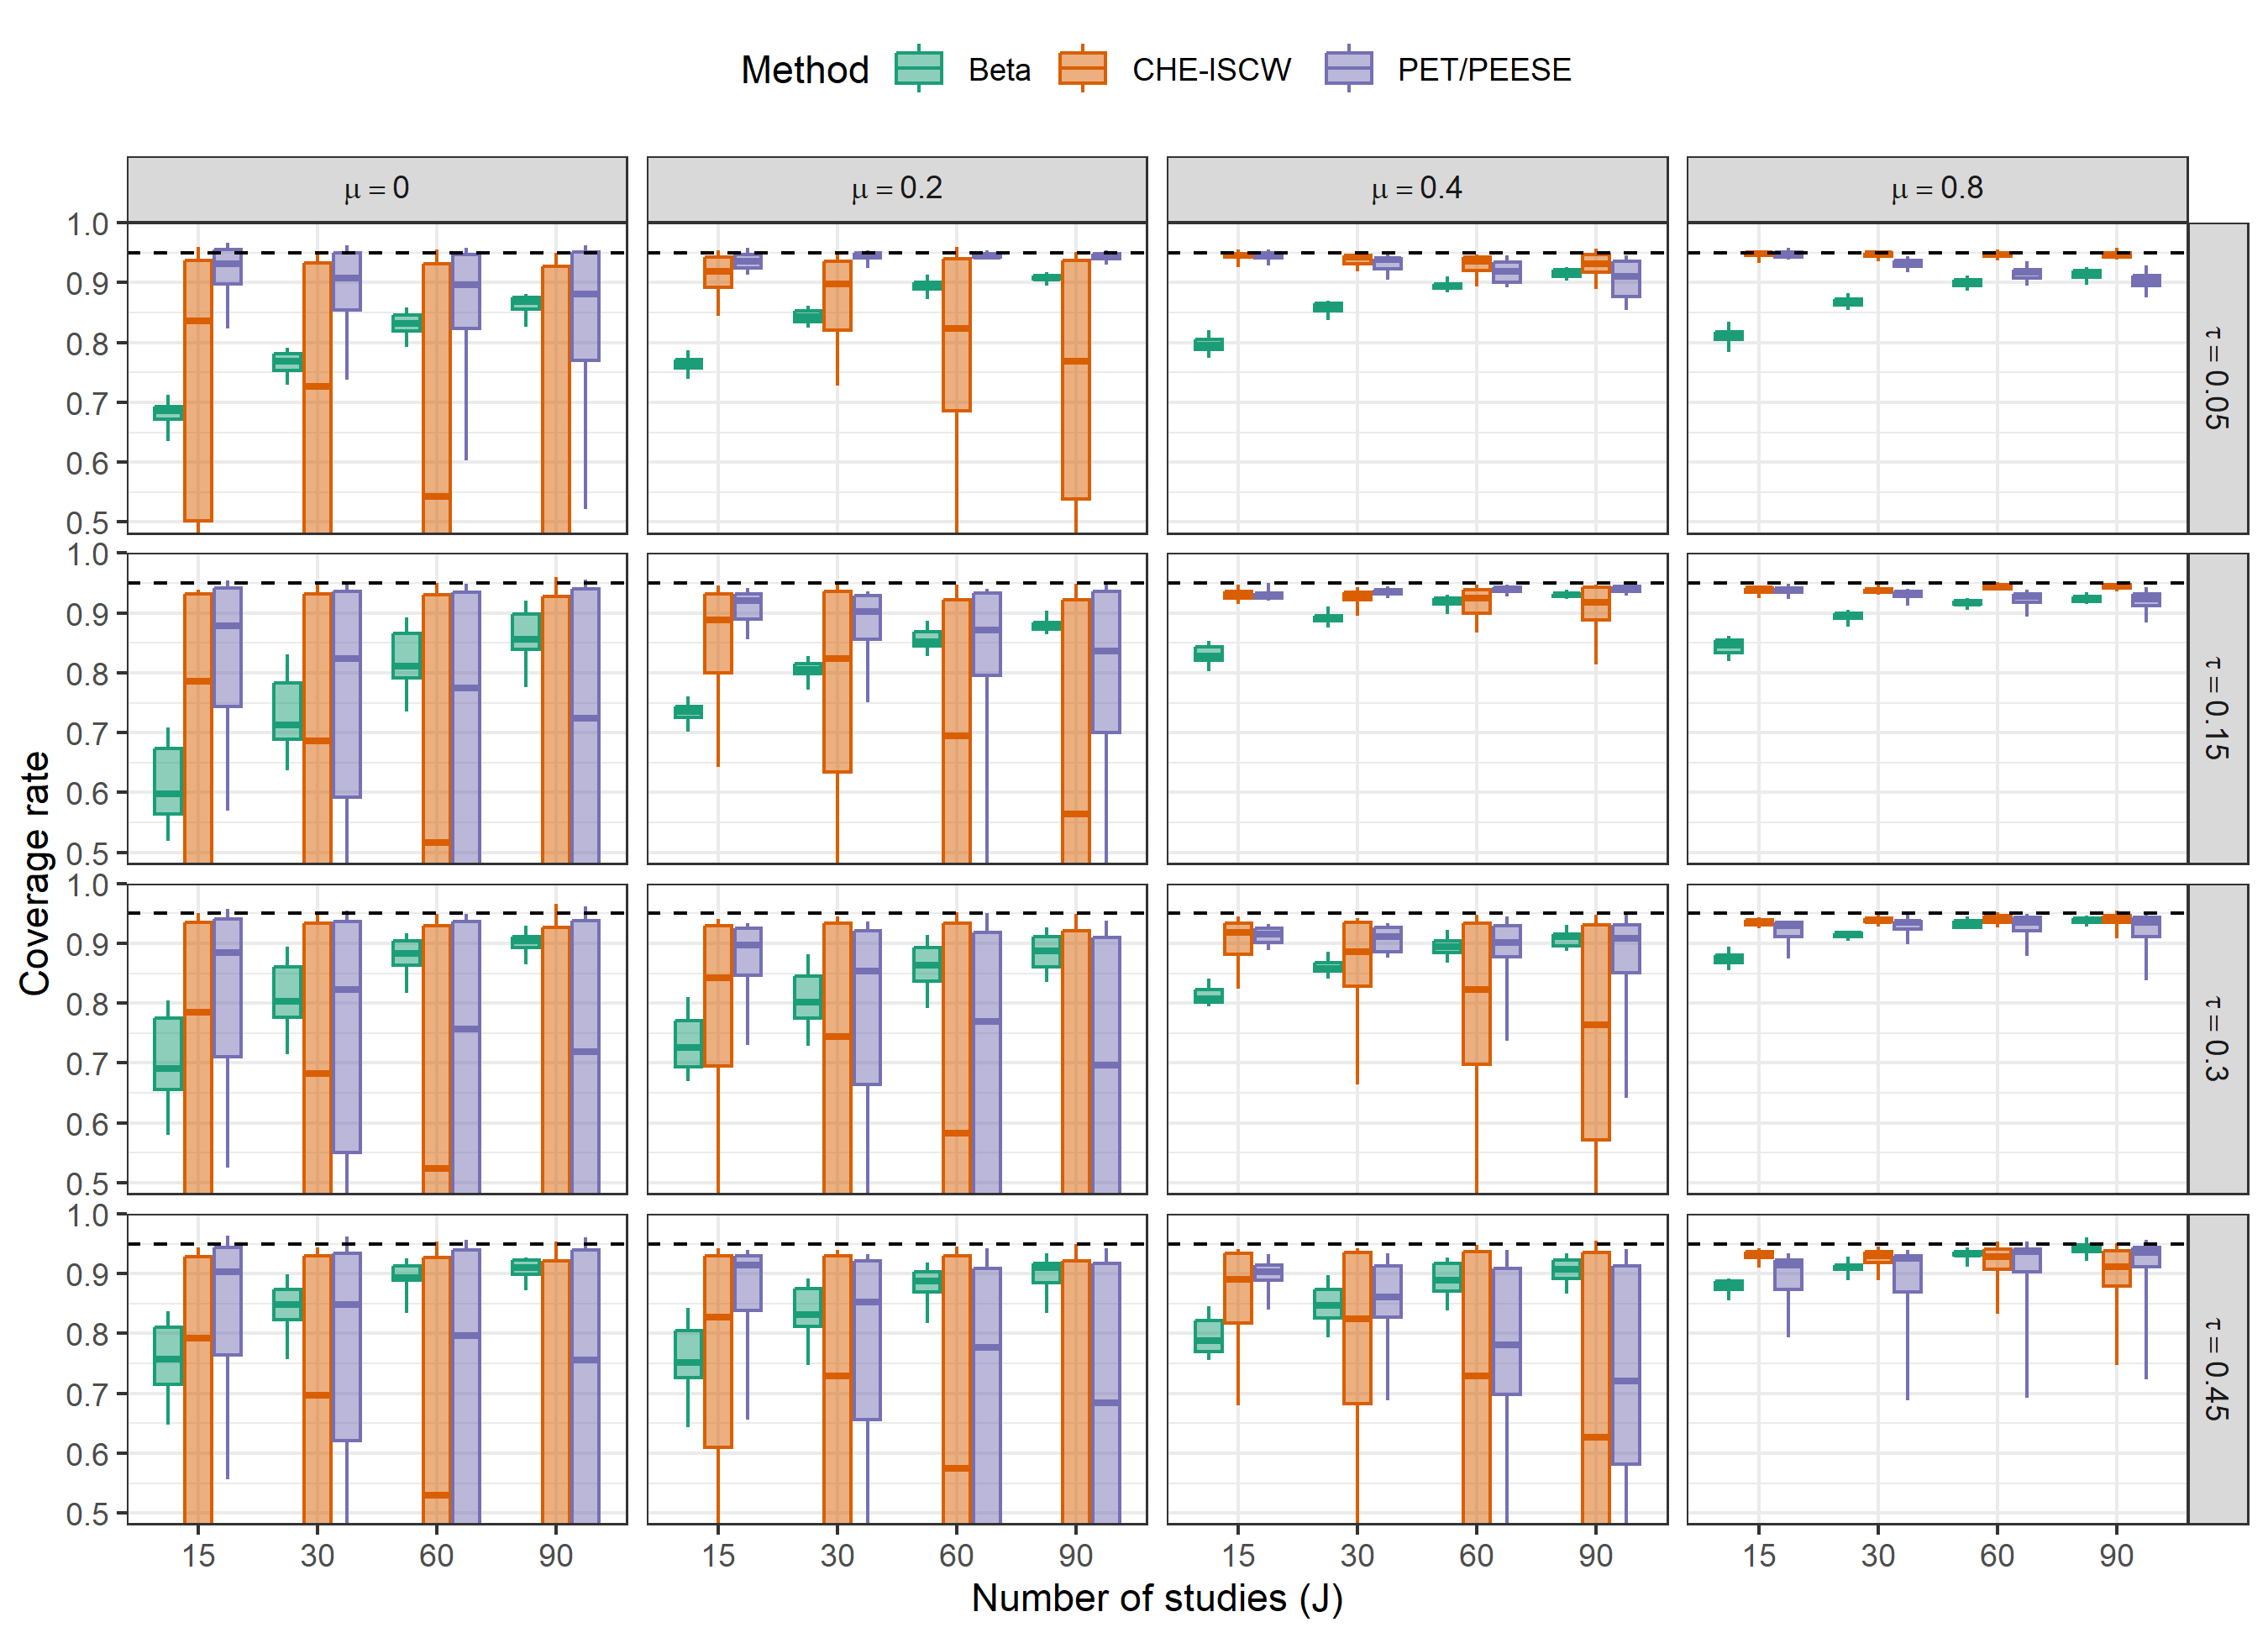
\includegraphics{beta-function-selection-models-with-dependent-effects_files/figure-latex/comparison-coverage-main-1} \caption{Coverage levels of confidence intervals for the average effect size based on cluster-robust variance approximations, by method, number of studies, average SMD, and between-study heterogeneity. Dashed lines correspond to the nominal confidence level of 0.95. Coverage rates of the CHE-ISCW and PET/PEESE intervals are not depicted when they fall below 0.5}\label{fig:comparison-coverage-main}
\end{sidewaysfigure}

Figure \ref{fig:comparison-coverage-main} shows the coverage rates of 95\% confidence intervals based on large-sample cluster-robust variance approximations for the three methods.\footnote{Note that the vertical axis of Figure \ref{fig:comparison-coverage-main} is restricted to the range {[}0.5, 1.0{]}, and coverage rates of the intervals based on CHE-ISCW and PET/PEESE are not depicted when they fall below 0.5. Supplementary Figure \ref{fig:comparison-coverage-full-main} depicts the full range of coverage rates.}
Across most conditions, coverage rates fall well below the nominal rate of 0.95 for all methods.
Coverage rates range from 0.52 to 0.97 for the beta-density selection model, from 0 to 0.97 for CHE-ISCW, and from 0.02 to 0.97 for PET/PEESE.
Coverage rates increase for all methods as the number of studies (\(J\)) increases, the average effect size increases (\(\mu\)), and heterogeneity decreases (\(\tau\)).
When heterogeneity is small (\(\tau \leq 0.15\)) and the average effect size is moderate to large (\(\mu \geq 0.4\)), CHE-ISCW has the highest coverage rates and the beta-density selection model has the lowest coverage rates.

It's important to note that the confidence intervals produced by the comparison methods are often severely miscalibrated. When CHE-ISCW and PET/PEESE are biased due to selective reporting, their intervals tend to be centered away from the true parameter. As a result, as the number of studies increases, the standard errors of the average effect size estimate-----and thus the interval widths-----shrink, causing coverage rates to decline sharply, in some cases approaching zero. This occurs more frequently when heterogeneity is moderate to large (\(\tau \geq 0.3\)) and the average effect size is small (\(\mu \leq 0.2\)), particularly for CHE-ISCW.

\begin{sidewaysfigure}
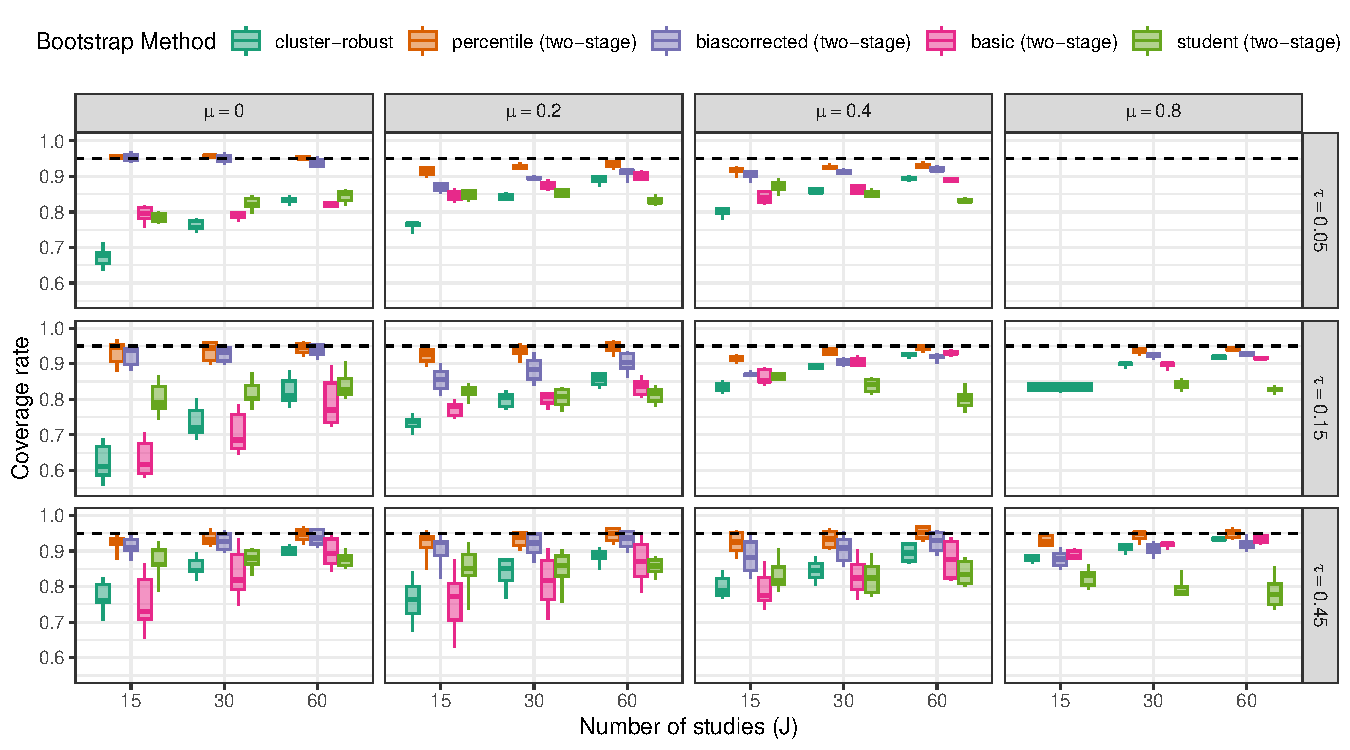
\includegraphics{beta-function-selection-models-with-dependent-effects_files/figure-latex/Beta-coverage-main-1} \caption{Coverage levels of confidence intervals for the average effect size estimated using the beta-density selection model, by bootstrap method, number of studies, average SMD, and between-study heterogeneity. Dashed lines correspond to the nominal confidence level of 0.95.}\label{fig:Beta-coverage-main}
\end{sidewaysfigure}

Figure \ref{fig:Beta-coverage-main} depicts the coverage rates of 95\% confidence intervals for the average effect size estimated using the beta-density selection model, comparing intervals based on the large-sample cluster-robust variance method to four two-stage bootstrapping methods (percentile, basic, studentized, and bias-corrected-and-accelerated).
Due to the computational demands of bootstrapping, we evaluated the bootstrap confidence intervals under a more limited range of data-generating conditions, including a maximum sample size of \(J = 60\).
Although no method achieves exact nominal coverage across all conditions, the percentile, studentized, and bias-corrected-and-accelerated bootstrap intervals consistently yield coverage rates comparable to-----or better than-----those based on the large-sample cluster-robust variance method.
Among these, the percentile bootstrap intervals performed best, achieving coverage above 90\% in nearly all conditions examined.

\subsection{Beta-Density Compared to One-Step and Two-Step Selection Models}\label{beta-density-compared-to-one-step-and-two-step-selection-models}

Convergence rates were higher for the step-function selection models than for the beta-density selection model. Both the one-step and two-step models had convergence rates of 99\% and above across all 1,280 conditions, while the beta-density selection model had convergence rates below 99\% for 40 of the 1,280 conditions.

\subsubsection{Bias}\label{bias-1}

\begin{sidewaysfigure}
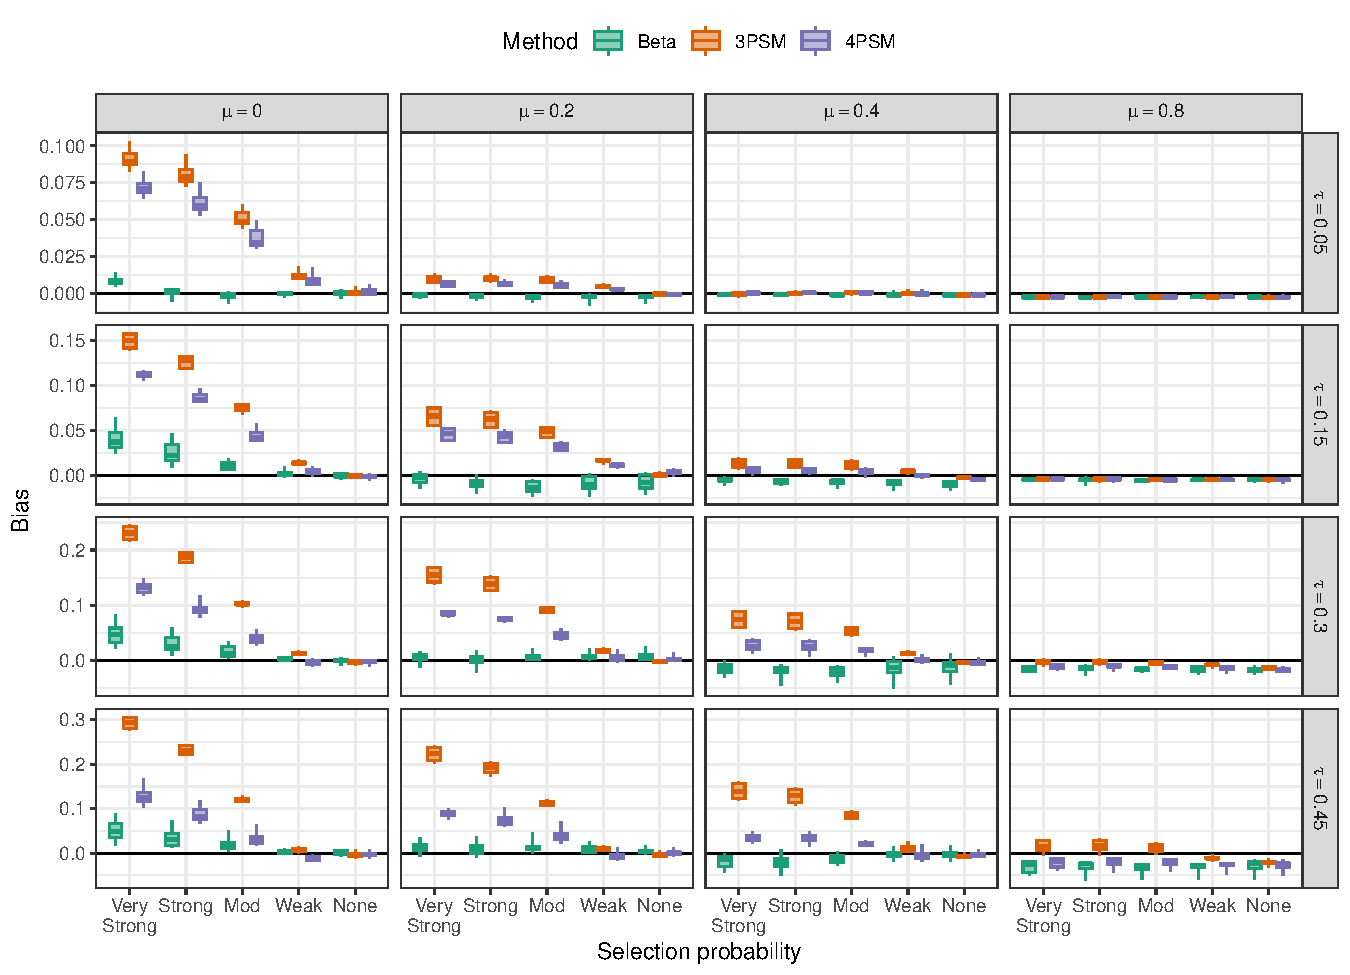
\includegraphics{beta-function-selection-models-with-dependent-effects_files/figure-latex/mu-bias-miss-1} \caption{Bias of the average effect size by method, selection probability, average SMD, and between-study heterogeneity}\label{fig:mu-bias-miss}
\end{sidewaysfigure}

Figure \ref{fig:mu-bias-miss} displays the bias for the three selection models. Across most conditions, bias is consistently closer to zero when the average effect size is estimated using the beta-density selection model compared to the step-function selection models. Among the step-function selection models, the two-step model generally outperforms the one-step model, though both are more prone to bias when the selection process is misspecified. The main exception occurs when average effect size is moderate to large \((\mu \geq 0.4)\) and heterogeneity is low \((\tau \leq 0.15)\), in which case all three models exhibit essentially zero bias. This pattern is consistent with the fact that the data were generated under a beta-density selection process and suggests that the step-function selection models, particularly the one-step model, are not robust to misspecification of the selection mechanism-----especially when selective reporting is moderate to strong or when average effect is not large \((\mu < 0.8)\).

\subsubsection{Scaled RMSE}\label{scaled-rmse-1}

\begin{sidewaysfigure}
\includegraphics{beta-function-selection-models-with-dependent-effects_files/figure-latex/mu-rmse-miss-1} \caption{Scaled root mean-squared error of the average effect size by method, selection probability, average SMD, and between-study heterogeneity}\label{fig:mu-rmse-miss}
\end{sidewaysfigure}

Figure \ref{fig:mu-rmse-miss} presents the scaled RMSE for the three selection models and highlights a clear bias--variance trade-off. When average effect size is zero and selective reporting is moderate to very strong, the results mirror the bias results pattern: the beta-density selection model outperforms the step-function selection models, and the two-step model performs better than the one-step model. However, the relative performance shifts under other conditions. For instance, when average effect size is \(\mu = 0.2\) and selective reporting is strong to very strong, the two-step model yields the lowest RMSE, even though it is misspecified. When average effect size is moderate or large (\(\mu \geq 0.2\)), or when \(\mu = 0.2\) and selective reporting is absent to moderate, the one-step model outperforms both alternatives, despite being misspecified. Scaled RMSE is similar across all three models when average effect size is moderate to large (\(\mu \geq 0.4\)) and heterogeneity is low (\(\tau \leq 0.15\)).

\subsubsection{Confidence Interval Coverage}\label{confidence-interval-coverage-1}

\begin{sidewaysfigure}
\includegraphics{beta-function-selection-models-with-dependent-effects_files/figure-latex/CML-coverage-miss-1} \caption{Coverage levels of confidence intervals for the average effect size based on two-stage bootstrap percentile intervals, by method, number of studies, average SMD, and between-study heterogeneity. Dashed lines correspond to the nominal confidence level of 0.95.}\label{fig:CML-coverage-miss}
\end{sidewaysfigure}

Figure \ref{fig:CML-coverage-miss} shows the coverage rates of 95\% confidence intervals based on two-stage bootstrap percentile intervals for the three models.
Based on the results above, we focus on the coverage rates of the two-stage bootstrap confidence intervals, particularly those constructed using percentile bootstrap methods, as they consistently yielded coverage rates better than those from the large-sample cluster-robust variance method.
Supplementary Figure \ref{fig:comparison-coverage-full-miss} depicts the coverage rates based on cluster-robust variance approximations.

The beta-density selection model achieves coverage rates at or near the nominal 0.95 level across all conditions.
The step-function selection models generally produce lower coverage rates, particularly when heterogeneity is moderate to large (\(\tau \geq 0.15\)) or average effect size is small (\(\mu \leq 0.2\)).
As with CHE-ISCW and PET/PEESE, the confidence intervals produced by the step-function selection models are often miscalibrated, due in part to underestimated standard errors, which result in overly narrow intervals.
Among the step-function selection models, coverage is generally higher for the two-step model than for the one-step model.

\subsubsection{Effect Size Variance}\label{effect-size-variance}

\section{Discussion}\label{discussion}

\section*{Author Contributions}\label{author-contributions}
\addcontentsline{toc}{section}{Author Contributions}

\textbf{MC:} Conceptualization, Methodology, Formal Analysis, Investigation, Writing - original draft, Writing - review \& editing, Project administration, Funding acquisition \textbf{JEP:} Conceptualization, Methodology, Software, Validation, Formal Analysis, Investigation, Resources, Writing - original draft, Writing - review \& editing

\section*{Funding}\label{funding}
\addcontentsline{toc}{section}{Funding}

This work was supported, in part, by the Institute of Educational Sciences, U.S. Department of Education through grant R305D220026 to the American Institutes of Research.
The opinions expressed are those of the authors and do not represent the views of the Institute of the U.S. Department of Education.

\section*{Acknowledgements}\label{acknowledgements}
\addcontentsline{toc}{section}{Acknowledgements}

\section*{Data and Replication Materials}\label{data-and-replication-materials}
\addcontentsline{toc}{section}{Data and Replication Materials}

Code and data for replicating the empirical example and the Monte Carlo simulation study are available on the Open Science Framework at .

\section*{Conflict of Interest Statement}\label{conflict-of-interest-statement}
\addcontentsline{toc}{section}{Conflict of Interest Statement}

The authors declare no conflicts of interest.

\section*{References}\label{references}
\addcontentsline{toc}{section}{References}

\begingroup

\phantomsection\label{refs}
\begin{CSLReferences}{1}{0}
\bibitem[\citeproctext]{ref-boos2000montecarlo}
Boos, D. D., \& Zhang, J. (2000). Monte carlo evaluation of resampling-based hypothesis tests. \emph{Journal of the American Statistical Association}, \emph{95}(450), 486--492. \url{https://doi.org/10.1080/01621459.2000.10474226}

\bibitem[\citeproctext]{ref-carter2019correcting}
Carter, E. C., Schönbrodt, F. D., Gervais, W. M., \& Hilgard, J. (2019). Correcting for bias in psychology: A comparison of meta-analytic methods. \emph{Advances in Methods and Practices in Psychological Science}, \emph{2}(2), 115--144.

\bibitem[\citeproctext]{ref-CHTC}
Center for High Throughput Computing. (2006). \emph{Center for high throughput computing}. Center for High Throughput Computing. \url{https://doi.org/10.21231/GNT1-HW21}

\bibitem[\citeproctext]{ref-chan2004empirical}
Chan, A.-W., Hróbjartsson, A., Haahr, M. T., Gøtzsche, P. C., \& Altman, D. G. (2004). Empirical evidence for selective reporting of outcomes in randomized trials: Comparison of protocols to published articles. \emph{Jama}, \emph{291}(20), 2457--2465.

\bibitem[\citeproctext]{ref-chen2024adapting}
Chen, M., \& Pustejovsky, J. E. (2024). \emph{Adapting methods for correcting selective reporting bias in meta-analysis of dependent effect sizes}. \url{https://doi.org/10.31222/osf.io/jq52s}

\bibitem[\citeproctext]{ref-citkowicz2017parsimonious}
Citkowicz, M., \& Vevea, J. L. (2017). {A parsimonious weight function for modeling publication bias}. \emph{Psychological Methods}, \emph{22}(1), 28--41. \url{https://doi.org/10.1037/met0000119}

\bibitem[\citeproctext]{ref-cox2004note}
Cox, D. R., \& Reid, N. (2004). A note on pseudolikelihood constructed from marginal densities. \emph{Biometrika}, \emph{91}(3), 729--737. \url{https://doi.org/10.1093/biomet/91.3.729}

\bibitem[\citeproctext]{ref-davison1997bootstrap}
Davison, A. C., \& Hinkley, D. V. (1997). \emph{Bootstrap methods and their applications}. Cambridge: Cambridge University Press.

\bibitem[\citeproctext]{ref-efron1987better}
Efron, B. (1987). Better bootstrap confidence intervals. \emph{Journal of the American Statistical Association}, \emph{82}(397), 171--185. \url{https://doi.org/10.1080/01621459.1987.10478410}

\bibitem[\citeproctext]{ref-field2007bootstrapping}
Field, C. A., \& Welsh, A. H. (2007). Bootstrapping clustered data. \emph{Journal of the Royal Statistical Society Series B: Statistical Methodology}, \emph{69}(3), 369--390. \url{https://doi.org/10.1111/j.1467-9868.2007.00593.x}

\bibitem[\citeproctext]{ref-franco2016underreporting}
Franco, A., Malhotra, N., \& Simonovits, G. (2016). Underreporting in psychology experiments: Evidence from a study registry. \emph{Social Psychological and Personality Science}, \emph{7}(1), 8--12. \url{https://doi.org/10.1177/1948550615598377}

\bibitem[\citeproctext]{ref-hedges1992modeling}
Hedges, L. V. (1992). Modeling publication selection effects in meta-analysis. \emph{Statistical Science}, \emph{7}(2), 246--255.

\bibitem[\citeproctext]{ref-hedges2017plausibility}
Hedges, L. V. (2017). Plausibility and influence in selection models: {A} comment on {Citkowicz} and {Vevea} (2017). \emph{Psychological Methods}, \emph{22}(1), 42--46. \url{https://doi.org/10.1037/met0000108}

\bibitem[\citeproctext]{ref-john2012measuring}
John, L. K., Loewenstein, G., \& Prelec, D. (2012). Measuring the prevalence of questionable research practices with incentives for truth telling. \emph{Psychological Science}, \emph{23}(5), 524--532.

\bibitem[\citeproctext]{ref-simhelpers}
Joshi, M., \& Pustejovsky, J. E. (2024). \emph{Simhelpers: Helper functions for simulation studies}. Retrieved from \url{https://meghapsimatrix.github.io/simhelpers/}

\bibitem[\citeproctext]{ref-kraft2020interpreting}
Kraft, M. A. (2020). Interpreting effect sizes of education interventions. \emph{Educational Researcher}, \emph{49}(4), 241--253.

\bibitem[\citeproctext]{ref-lancee2017outcome}
Lancee, M., Lemmens, C., Kahn, R., Vinkers, C., \& Luykx, J. (2017). Outcome reporting bias in randomized-controlled trials investigating antipsychotic drugs. \emph{Translational Psychiatry}, \emph{7}(9), e1232--e1232.

\bibitem[\citeproctext]{ref-leedouw2008resampling}
Leeden, R. V. D., Meijer, E., \& Busing, F. M. T. A. (2008). Resampling multilevel models. In J. D. Leeuw \& E. Meijer (Eds.), \emph{Handbook of {Multilevel} {Analysis}} (pp. 401--433). New York, NY: Springer New York. \url{https://doi.org/10.1007/978-0-387-73186-5_11}

\bibitem[\citeproctext]{ref-lindsay1988composite}
Lindsay, B. G. (1988). Composite likelihood methods. In N. U. Prabhu (Ed.), \emph{Contemporary {Mathematics}} (Vol. 80, pp. 221--239). Providence, Rhode Island: American Mathematical Society. \url{https://doi.org/10.1090/conm/080/999014}

\bibitem[\citeproctext]{ref-marksanglin2020historical}
Marks‐Anglin, A., \& Chen, Y. (2020). A historical review of publication bias. \emph{Research Synthesis Methods}, \emph{11}(6), 725--742. \url{https://doi.org/10.1002/jrsm.1452}

\bibitem[\citeproctext]{ref-optimx}
Nash, J. C., \& Varadhan, R. (2011). Unifying optimization algorithms to aid software system users: {optimx} for {R}. \emph{Journal of Statistical Software}, \emph{43}(9), 1--14. \url{https://doi.org/10.18637/jss.v043.i09}

\bibitem[\citeproctext]{ref-oBoyle2017chrysalis}
O'Boyle Jr, E. H., Banks, G. C., \& Gonzalez-Mulé, E. (2017). The chrysalis effect: How ugly initial results metamorphosize into beautiful articles. \emph{Journal of Management}, \emph{43}(2), 376--399.

\bibitem[\citeproctext]{ref-pigott2013outcome}
Pigott, T. D., Valentine, J. C., Polanin, J. R., Williams, R. T., \& Canada, D. D. (2013). Outcome-reporting bias in education research. \emph{Educational Researcher}, \emph{42}(8), 424--432.

\bibitem[\citeproctext]{ref-clubSandwich}
Pustejovsky, J. E. (2024). \emph{clubSandwich: Cluster-robust (sandwich) variance estimators with small-sample corrections}. Retrieved from \url{https://CRAN.R-project.org/package=clubSandwich}

\bibitem[\citeproctext]{ref-pustejovsky2025step}
Pustejovsky, J. E., Citkowicz, M., \& Joshi, M. (2025). Estimation and inference for step-function selection models in meta-analysis with dependent effects. \emph{Journal Name}.

\bibitem[\citeproctext]{ref-metaselection}
Pustejovsky, J. E., Joshi, M., \& Citkowicz, M. (2025). \emph{Metaselection: Meta-analytic selection models with cluster-robust and cluster-bootstrap standard errors for dependent effect size estimates}. Retrieved from \url{https://github.com/jepusto/metaselection}

\bibitem[\citeproctext]{ref-rcoreteam}
R Core Team. (2023). \emph{R: A language and environment for statistical computing}. Vienna, Austria: R Foundation for Statistical Computing. Retrieved from \url{https://www.R-project.org/}

\bibitem[\citeproctext]{ref-Rothstein2005publication}
Rothstein, H. R., Sutton, A. J., \& Borenstein, M. (2005). Publication bias in meta-analysis. In H. R. Rothstein, A. J. Sutton, \& M. Borenstein (Eds.), \emph{Publication {Bias} in {Meta-Analysis}: {Prevention}, {Assessment}, and {Adjustments}} (pp. 1--7). {West Sussex, England}: {John Wiley \& Sons}. \url{https://doi.org/10.1002/0470870168}

\bibitem[\citeproctext]{ref-rubin1981bayesian}
Rubin, D. B. (1981). The {Bayesian} bootstrap. \emph{The Annals of Statistics}, \emph{9}(1). \url{https://doi.org/10.1214/aos/1176345338}

\bibitem[\citeproctext]{ref-stanley2014meta}
Stanley, T. D., \& Doucouliagos, H. (2014). Meta-regression approximations to reduce publication selection bias. \emph{Research Synthesis Methods}, \emph{5}(1), 60--78.

\bibitem[\citeproctext]{ref-taylor2018science}
Taylor, J. A., Kowalski, S. M., Polanin, J. R., Askinas, K., Stuhlsatz, M. A. M., Wilson, C. D., \ldots{} Wilson, S. J. (2018). Investigating science education effect sizes: Implications for power analyses and programmatic decisions. \emph{AERA Open}, \emph{4}(3), 1--19. \url{https://doi.org/10.1177/2332858418791991}

\bibitem[\citeproctext]{ref-Terrin2003heterogeneity}
Terrin, N., Schmid, C. H., Lau, J., \& Olkin, I. (2003). Adjusting for publication bias in the presence of heterogeneity. \emph{Statistics in Medicine}, \emph{22}(13), 2113--2126. \url{https://doi.org/10.1002/sim.1461}

\bibitem[\citeproctext]{ref-tipton2019current}
Tipton, E., Pustejovsky, J. E., \& Ahmadi, H. (2019). Current practices in meta-regression in psychology, education, and medicine. \emph{Research Synthesis Methods}, \emph{10}(2), 180--194.

\bibitem[\citeproctext]{ref-varin2008composite}
Varin, C. (2008). On composite marginal likelihoods. \emph{AStA Advances in Statistical Analysis}, \emph{92}(1), 1--28. \url{https://doi.org/10.1007/s10182-008-0060-7}

\bibitem[\citeproctext]{ref-vevea1995general}
Vevea, J. L., \& Hedges, L. V. (1995). A general linear model for estimating effect size in the presence of publication bias. \emph{Psychometrika}, \emph{60}(3), 419--435. \url{https://doi.org/10.1007/BF02294384}

\bibitem[\citeproctext]{ref-Viechtbauer2010conducting}
Viechtbauer, W. (2010). {Conducting meta-analyses in R with the metafor package}. \emph{Journal of Statistical Software}, \emph{36}(3), 1--48.

\bibitem[\citeproctext]{ref-tidyverse}
Wickham, H., Averick, M., Bryan, J., Chang, W., McGowan, L. D., François, R., \ldots{} Yutani, H. (2019). Welcome to the {tidyverse}. \emph{Journal of Open Source Software}, \emph{4}(43), 1686. \url{https://doi.org/10.21105/joss.01686}

\bibitem[\citeproctext]{ref-Wolf2023making}
Wolf, B., \& Harbatkin, E. (2023). Making sense of effect sizes: Systematic differences in intervention effect sizes by outcome measure type. \emph{Journal of Research on Educational Effectiveness}, \emph{16}(1), 134--161. \url{https://doi.org/10.1080/19345747.2022.2071364}

\bibitem[\citeproctext]{ref-xu2020applications}
Xu, L., Gotwalt, C., Hong, Y., King, C. B., \& Meeker, W. Q. (2020). Applications of the fractional-random-weight bootstrap. \emph{The American Statistician}, \emph{74}(4), 345--358. \url{https://doi.org/10.1080/00031305.2020.1731599}

\end{CSLReferences}

\endgroup

\appendix


\section{Beta-Function Selection Model Compared to CHE-ISCW and PET/PEESE}\label{beta-function-selection-model-compared-to-che-iscw-and-petpeese}

\subsection{\texorpdfstring{Additional simulation results for methods of estimating the average effect size \((\mu)\)}{Additional simulation results for methods of estimating the average effect size (\textbackslash mu)}}\label{mu-simulation-results-main}

\begin{sidewaysfigure}
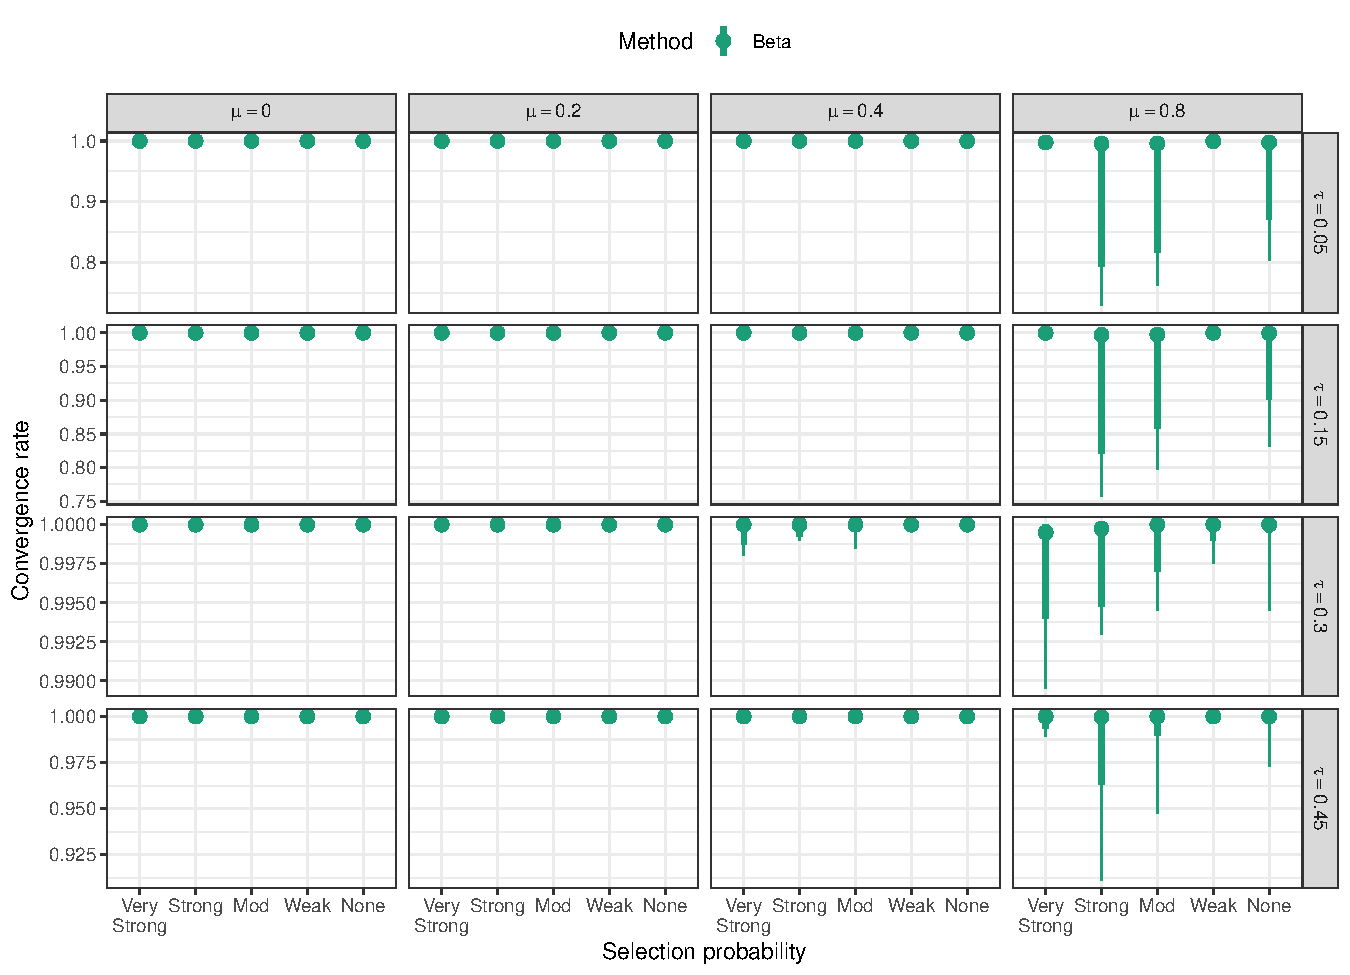
\includegraphics{beta-function-selection-models-with-dependent-effects_files/figure-latex/convergence-rates-main-1} \caption{Convergence rates of the beta-function selection model by selection probability, average SMD, and between-study heterogeneity. Points correspond to median convergence rates; thin lines correspond to range of convergence rates; thick lines correspond to inter-decile range.}\label{fig:convergence-rates-main}
\end{sidewaysfigure}

\begin{sidewaysfigure}
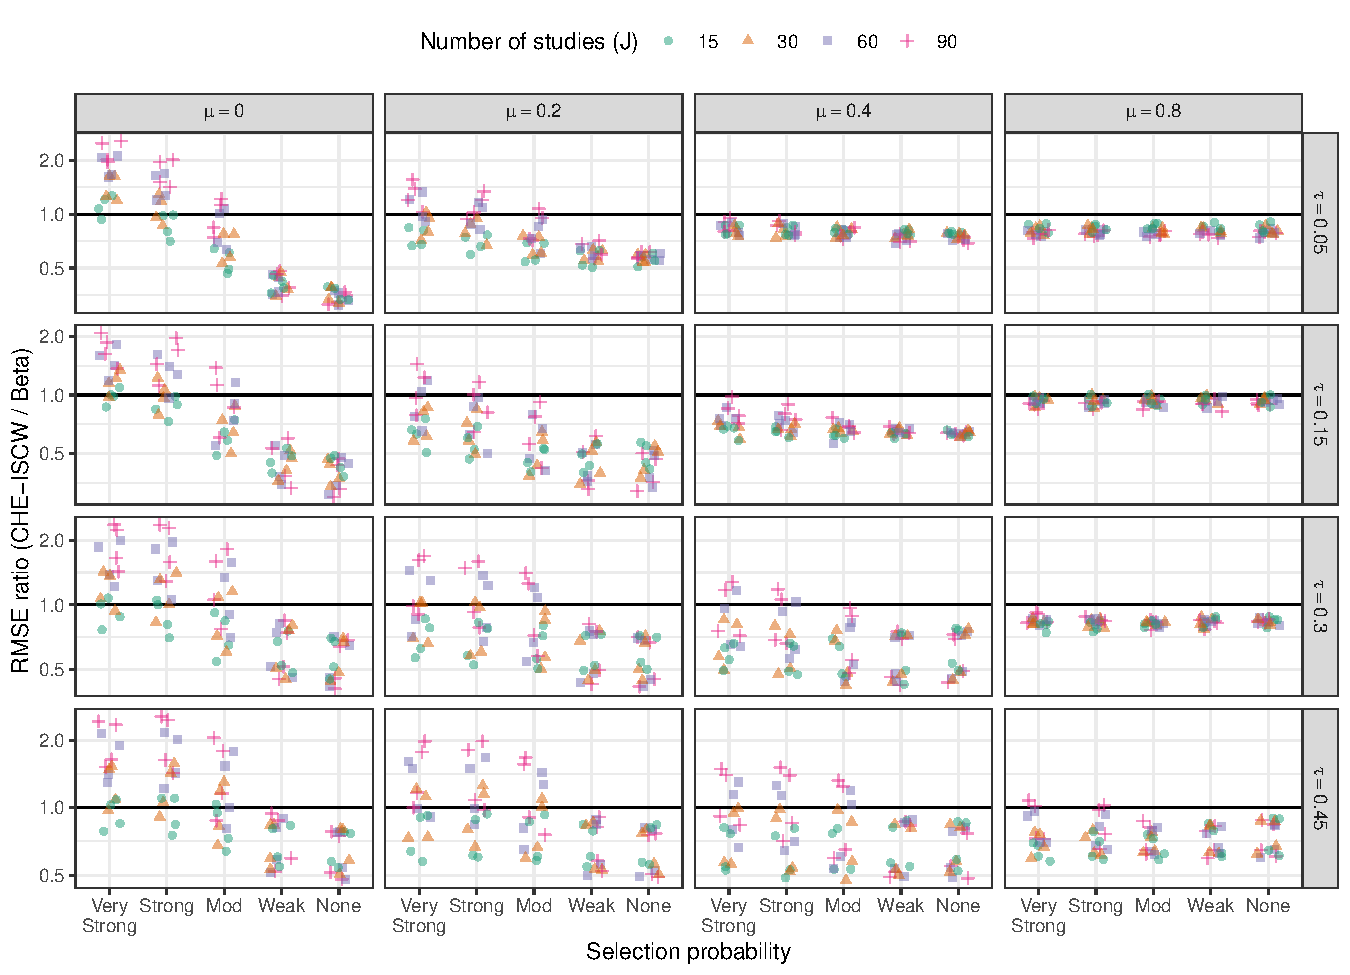
\includegraphics{beta-function-selection-models-with-dependent-effects_files/figure-latex/rmse-CHE-Beta-main-1} \caption{Ratio of root mean-squared error for CHE-ISCW estimator to root mean-squared error of CML estimator by selection probability, number of studies, average SMD, and between-study heterogeneity}\label{fig:rmse-CHE-Beta-main}
\end{sidewaysfigure}

\begin{sidewaysfigure}
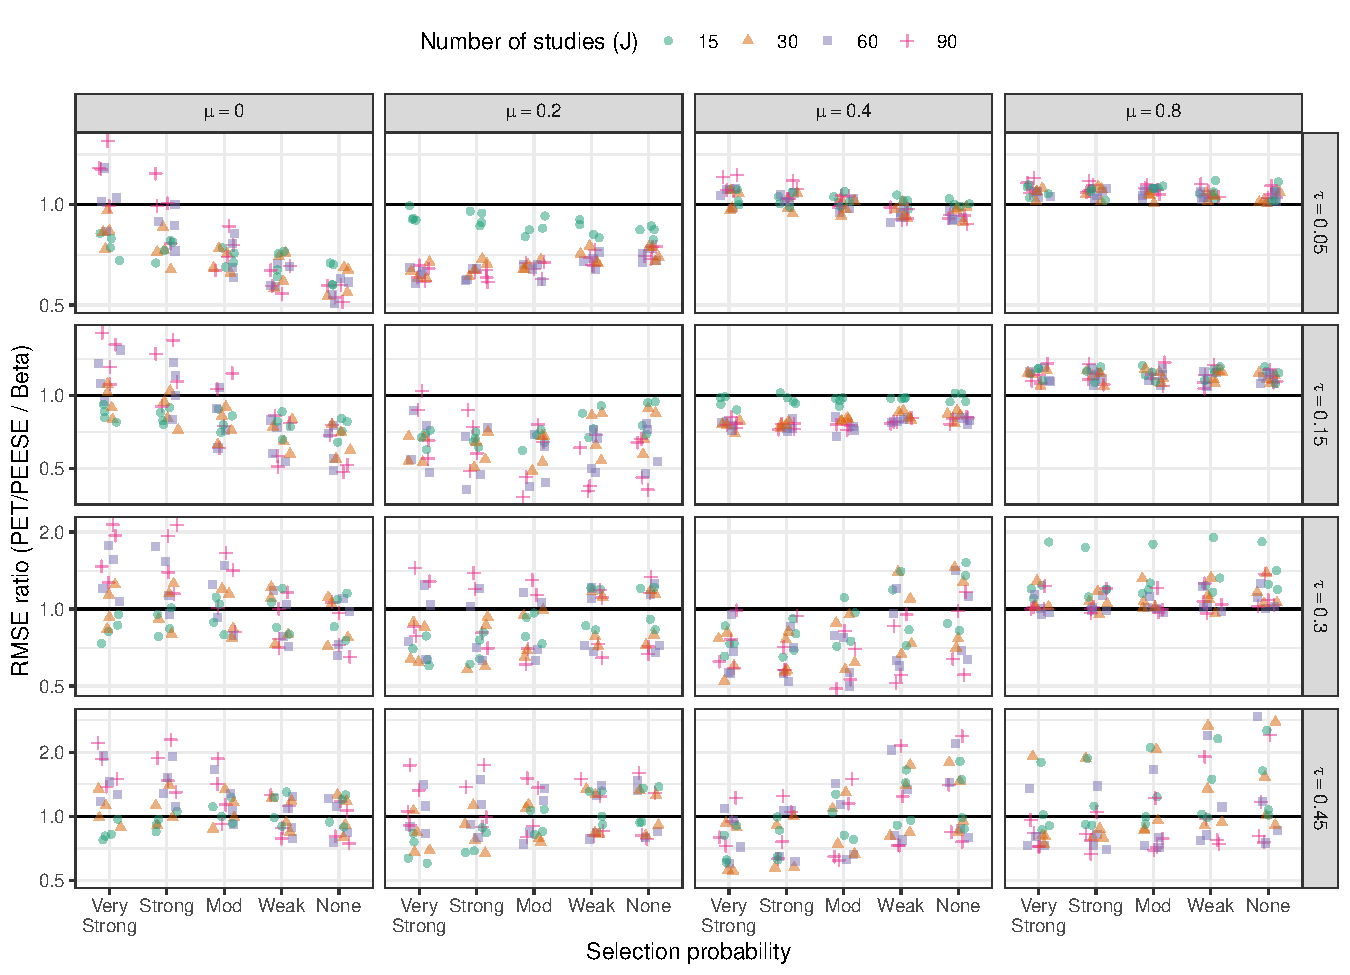
\includegraphics{beta-function-selection-models-with-dependent-effects_files/figure-latex/rmse-PET-Beta-main-1} \caption{Ratio of root mean-squared error for PET/PEESE estimator to root mean-squared error of CML estimator by selection probability, number of studies, average SMD, and between-study heterogeneity}\label{fig:rmse-PET-Beta-main}
\end{sidewaysfigure}

\begin{sidewaysfigure}
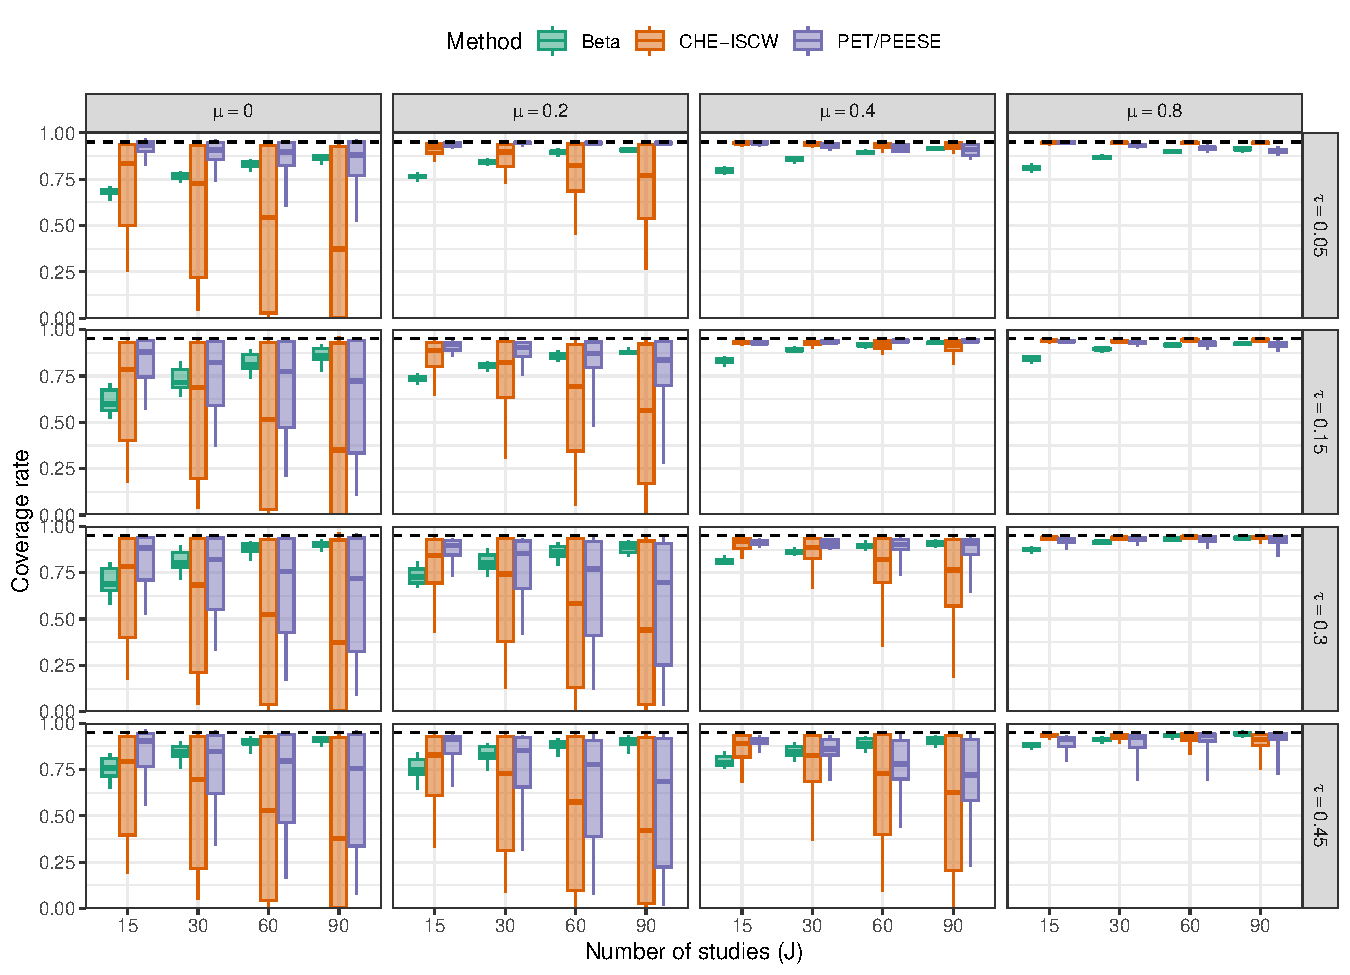
\includegraphics{beta-function-selection-models-with-dependent-effects_files/figure-latex/comparison-coverage-full-main-1} \caption{Coverage levels of confidence intervals for the average effect size based on cluster-robust variance approximations, by method, number of studies, average SMD, and between-study heterogeneity. Dashed lines correspond to the nominal confidence level of 0.95.}\label{fig:comparison-coverage-full-main}
\end{sidewaysfigure}

\section{Beta-Function Selection Model Compared to 3PSM and 4PSM Step-Function Selection Models}\label{beta-function-selection-model-compared-to-3psm-and-4psm-step-function-selection-models}

\subsection{\texorpdfstring{Additional simulation results for methods of estimating the average effect size \((\mu)\)}{Additional simulation results for methods of estimating the average effect size (\textbackslash mu)}}\label{mu-simulation-results-miss}

\begin{sidewaysfigure}
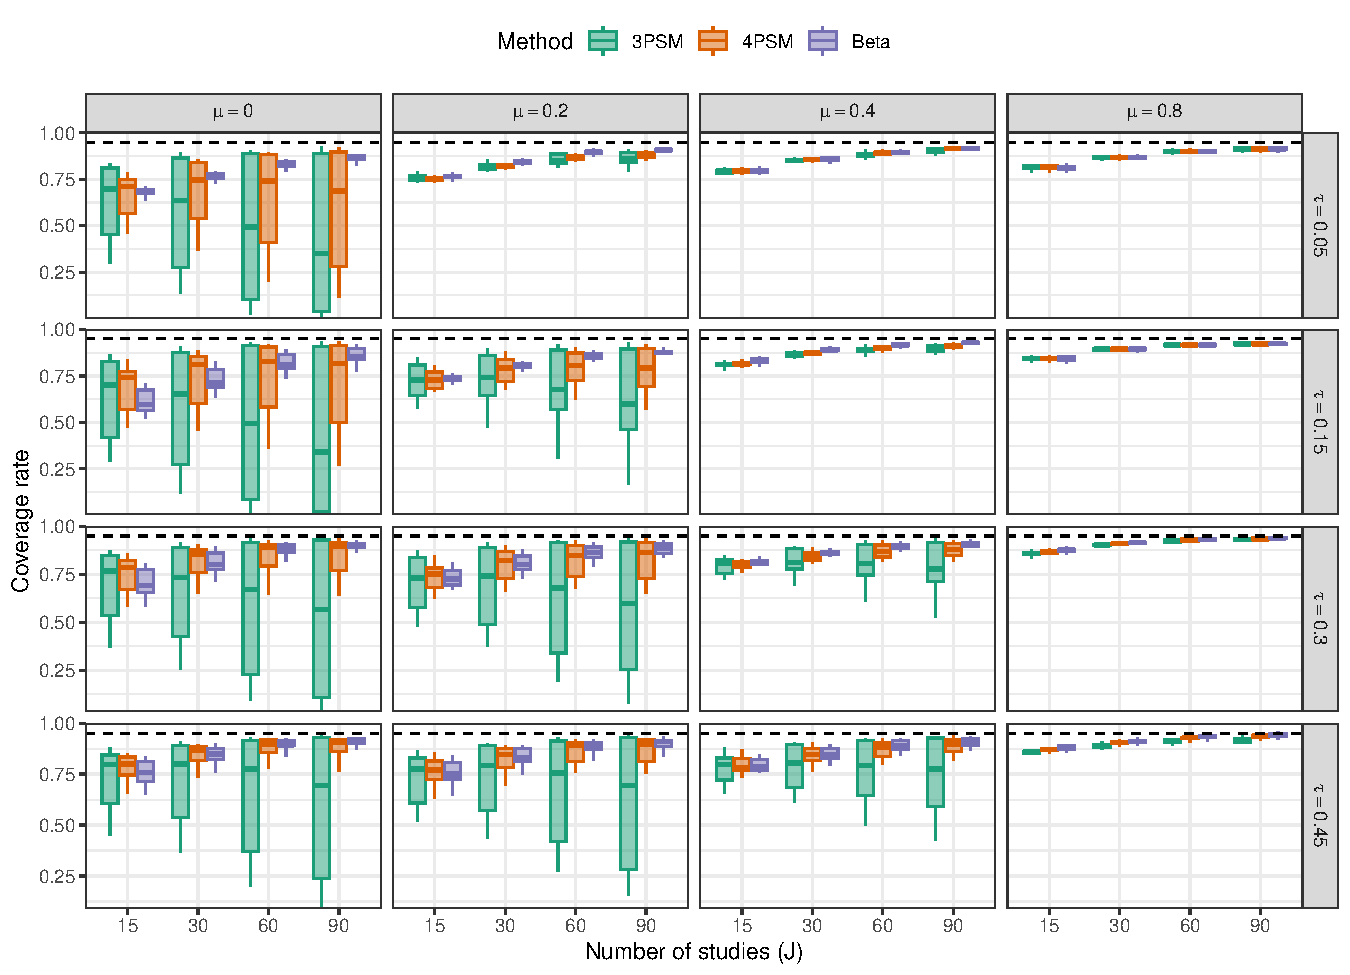
\includegraphics{beta-function-selection-models-with-dependent-effects_files/figure-latex/comparison-coverage-full-miss-1} \caption{Coverage levels of confidence intervals for the average effect size based on cluster-robust variance approximations, by method, number of studies, average SMD, and between-study heterogeneity. Dashed lines correspond to the nominal confidence level of 0.95.}\label{fig:comparison-coverage-full-miss}
\end{sidewaysfigure}


\end{document}
